\chapter{Method}
The design and prototype iterations of the haptic metronome are discussed extensively throughout Appendix \ref{designReq} along with a parts list and schematic of the hardware builds.\footnote{All of the code is open source and readily available at \url{https://github.com/afaintillusion/he-sm}}

This chapter outlines each test case and describes the motivation behind the test plan. Furthermore, it briefly delves into the test suite design and calculates a round-trip latency of the system in order to find a close approximation of relative accuracy. The hope is to establish a level of confidence in the precise time dependent information.

The overall test principle was derived from traditional sensorimotor synchronization tasks in which a user is asked to tap to a corresponding stimulus. The asynchrony was tracked and plotted along with the \textit{PCR} and any missed taps. Since the haptic domain is of primary focus, the auditory modality functions primarily as a benchmark or baseline foundation. The work presented in \ref{visualMet} covers the idea of the interstitial beat occupying the visual domain and as such will not be re-evaluated here.

Each test case is defined and presented in \ref{testPlan}. The overall software development process is detailed in \ref{development}. The test suite is discussed in \ref{tap_arduino} and latency calculated in \ref{latencyCalc}.

\section{Test Plan} \label{testPlan}
Testing was divided into two major sections, \textbf{Steady} and \textbf{Dynamic}, implying either an \textit{isochronous} or a \textit{non-isochronous} pulse respectively. While structurally identical, the dynamic tests however focussed on rubato within a range starting at the predefined BPM and rising or falling within a specified window (maximum span of +/- 15 bpm). The chosen tempi parallels slow walking to running gaits spanning a range of 45-180 beats per minute.

Each section has three subsections centered around either an audible metronome tone (\textbf{A1, A3}), musical note (\textbf{A2, A4}), and lastly the haptic modality (\textbf{H1, H2}). Subsections were further broken down into \textbf{a} and \textbf{b}, denoting either \textit{discrete} or \textit{interstitial} (\textit{continuous}) mode of operation. A breakdown of the test plan is shown in Figure \ref{fig:TestPlan}. The data analysis in Chapter \ref{DataAnalysis} will frequently reference this table as a legend.

As discussed in Appendix \ref{designReq}, the haptic was designed with two operating modes in mind, discrete and continuous. These modes were programmatically controlled to match the desired test cases, extensively explained in section \ref{development}.
\begin{table}[t]
    \centering
    \resizebox{\textwidth}{!}{%
        \begin{tabular}{cclllcclll}
        \hline
        \multicolumn{10}{c}{\cellcolor[HTML]{000000}{\color[HTML]{FFFFFF} Steady}} \\ \hline
        \multicolumn{3}{c}{Discrete} & BPM & \multicolumn{1}{l|}{Runtime (sec)} & \multicolumn{3}{c}{Interstitial} & BPM & Runtime (sec) \\ \hline
        &  & i. & 45 & \multicolumn{1}{l|}{20} &  &  & i. & 45 & 30 \\
        &  & ii. & 90 & \multicolumn{1}{l|}{20} &  &  & ii. & 90 & 16 \\
        &  & iii. & 135 & \multicolumn{1}{l|}{20} &  &  & iii. & 135 & 11 \\
        \multirow{-4}{*}{A1a} & \multirow{-4}{*}{click} & iv. & 180 & \multicolumn{1}{l|}{20} & \multirow{-4}{*}{A1b} & \multirow{-4}{*}{legato chime (swing click)} & iv. & 180 & 8 \\ \hline
        &  & i. & 45 & \multicolumn{1}{l|}{32} &  &  & i. & 45 & 32 \\
        &  & ii. & 90 & \multicolumn{1}{l|}{16} &  &  & ii. & 90 & 16 \\
        &  & iii. & 135 & \multicolumn{1}{l|}{11} &  &  & iii. & 135 & 11 \\
        \multirow{-4}{*}{A2a} & \multirow{-4}{*}{staccato music (melody)} & iv. & 180 & \multicolumn{1}{l|}{8} & \multirow{-4}{*}{A2b} & \multirow{-4}{*}{legato music (melody)} & iv. & 180 & 8 \\ \hline
        &  & i. & 45 & \multicolumn{1}{l|}{15} &  &  & i. & 45 & 15 \\
        &  & ii. & 90 & \multicolumn{1}{l|}{15} &  &  & ii. & 90 & 15 \\
        &  & iii. & 135 & \multicolumn{1}{l|}{15} &  &  & iii. & 135 & 15 \\
        \multirow{-4}{*}{H1a} & \multirow{-4}{*}{poke / all on (instantaneous)} & iv. & 180 & \multicolumn{1}{l|}{15} & \multirow{-4}{*}{H1b} & \multirow{-4}{*}{oscillate down and back up} & iv. & 180 & 15 \\ \hline
        \multicolumn{10}{c}{\cellcolor[HTML]{000000}{\color[HTML]{FFFFFF} Dynamic}} \\ \hline
        \multicolumn{3}{c}{Discrete} & BPM & \multicolumn{1}{l|}{Runtime (sec)} & \multicolumn{3}{c}{Interstitial} & BPM & Runtime (sec) \\ \hline
        &  & i. & 45 +/- 15 & \multicolumn{1}{l|}{20} &  &  & i. & 45 +/- 15 & 20 \\
        &  & ii. & 90 +/- 15 & \multicolumn{1}{l|}{10} &  &  & ii. & 90 +/- 15 & 10 \\
        &  & iii. & 135 +/- 15 & \multicolumn{1}{l|}{10} &  &  & iii. & 135 +/- 15 & 10 \\
        \multirow{-4}{*}{A3a} & \multirow{-4}{*}{click} & iv. & 180 +/- 15 & \multicolumn{1}{l|}{10} & \multirow{-4}{*}{A3b} & \multirow{-4}{*}{legato chime (swing click)} & iv. & 180 +/- 15 & 10 \\ \hline
        &  & i. & 45 +/- 15 & \multicolumn{1}{l|}{30} &  &  & i. & 45 +/- 15 & 30 \\
        &  & ii. & 90 +/- 15 & \multicolumn{1}{l|}{15} &  &  & ii. & 90 +/- 15 & 15 \\
        &  & iii. & 135 +/- 15 & \multicolumn{1}{l|}{10} &  &  & iii. & 135 +/- 15 & 10 \\
        \multirow{-4}{*}{A4a} & \multirow{-4}{*}{staccato music (melody)} & iv. & 180 +/- 15 & \multicolumn{1}{l|}{10} & \multirow{-4}{*}{A4b} & \multirow{-4}{*}{legato music (melody)} & iv. & 180 +/- 15 & 10 \\ \hline
        &  & i. & 45 +/- 10 & \multicolumn{1}{l|}{15} &  &  & i. & 45 +/- 10 & 15 \\
        &  & ii. & 90 +/- 5 & \multicolumn{1}{l|}{15} &  &  & ii. & 90 +/- 5 & 15 \\
        &  & iii. & 135 +/- 3 & \multicolumn{1}{l|}{15} &  &  & iii. & 135 +/- 3 & 15 \\
        \multirow{-4}{*}{H2a} & \multirow{-4}{*}{poke / all on (instantaneous)} & iv. & 180 +/- 1 & \multicolumn{1}{l|}{15} & \multirow{-4}{*}{H2b} & \multirow{-4}{*}{oscillate down and back up} & iv. & 180 +/- 1 & 15 \\ \hline
        \end{tabular}%
    }
    \caption{Test Plan}
    \label{fig:TestPlan}
\end{table}

\subsection{Subjects}
Out of 18 subjects tested, 16 were parsed to equivalently divide the groups into 8 professionals and 8 amateurs/non-musicians. Usernames were anonymized into User ID's using a cumulative char to int conversion method. A breakdown of the grouping per instrumentation is shown in Table \ref{fig:SubjectTable}.
\begin{table}[t]
    \centering
    \resizebox{.5\textwidth}{!}{%
    \begin{tabular}{|l|l|l|}
    \hline
    \rowcolor[HTML]{000000} 
    {\color[HTML]{FFFFFF} Group} & {\color[HTML]{FFFFFF} Instrument} & {\color[HTML]{FFFFFF} User ID} \\ \hline
     & Bass & 729 \\ \cline{2-3} 
     & DJ & 390 \\ \cline{2-3} 
     & Piano & 399 \\ \cline{2-3} 
    \multirow{-4}{*}{Amateur} & Voice & 379 \\ \hline
     &  & 486 \\ \cline{3-3} 
     &  & 514 \\ \cline{3-3} 
     & \multirow{-3}{*}{None} & 932 \\ \cline{2-3} 
    \multirow{-4}{*}{Neither} & Piano & 394 \\ \hline
     &  & 410 \\ \cline{3-3} 
     &  & 591 \\ \cline{3-3} 
     & \multirow{-3}{*}{Flute} & 824 \\ \cline{2-3} 
     &  & 367 \\ \cline{3-3} 
     &  & 506 \\ \cline{3-3} 
     &  & 521 \\ \cline{3-3} 
     & \multirow{-4}{*}{Percussion} & 552 \\ \cline{2-3} 
    \multirow{-8}{*}{Professional} & Piano & 510 \\ \hline
    \end{tabular}%
    }
    \caption{Subject Grouping}
    \label{fig:SubjectTable}
\end{table}

\subsection{Audio File Generation}
All tracks were rendered using the digital audio workstation (DAW) \textit{Logic Pro X} as \textit{.wav} files at a 44.1kHz sample rate with 16 bit resolution.

\subsubsection{Metronomic click and legato chime}
\textbf{A1a} and \textbf{A3a} required a standard metronomic pulse. This was accomplished using the default Klopfgeist (metronome) plugin from Logic Pro X. No additional tuning was modified and the tonality was left at 0.83 of unity.

\begin{figure}[H]
    \centering
    \caption{Modified click parameters for interstitial tests.}
        \subfloat[Modified metronome]{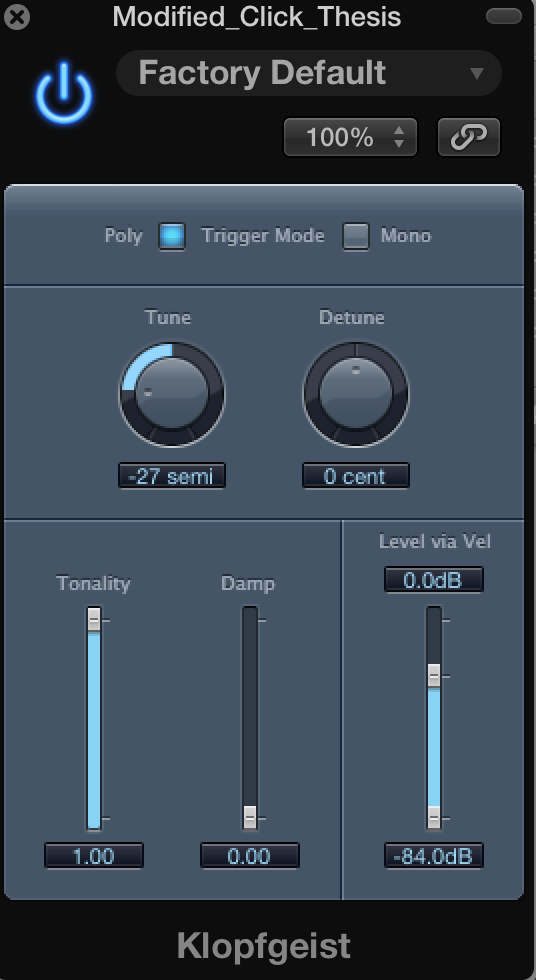
\includegraphics[width=0.25\columnwidth]{Klopfgeist_Modified}}
        \qquad
        \subfloat[Superimposed tremolo]{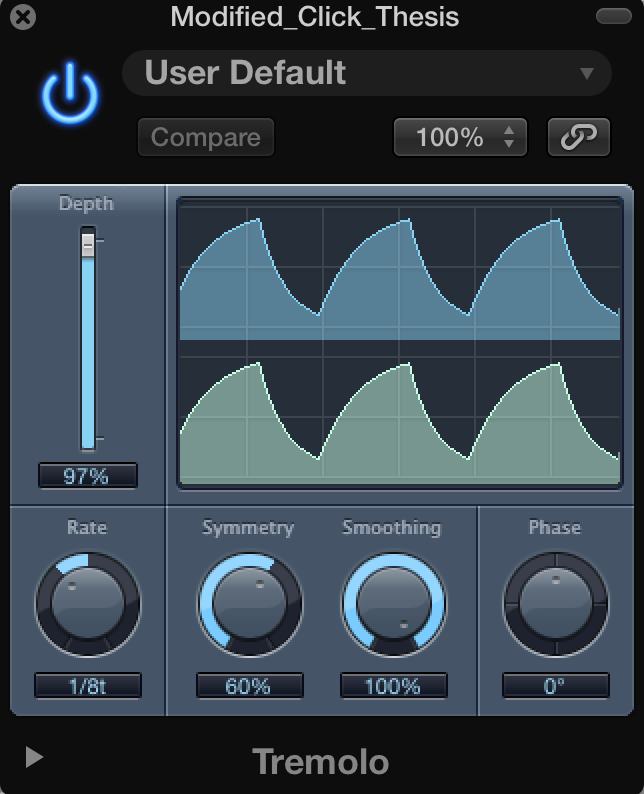
\includegraphics[width=0.4\columnwidth]{Tremolo}}
        \qquad
        \subfloat[Equalized tone]{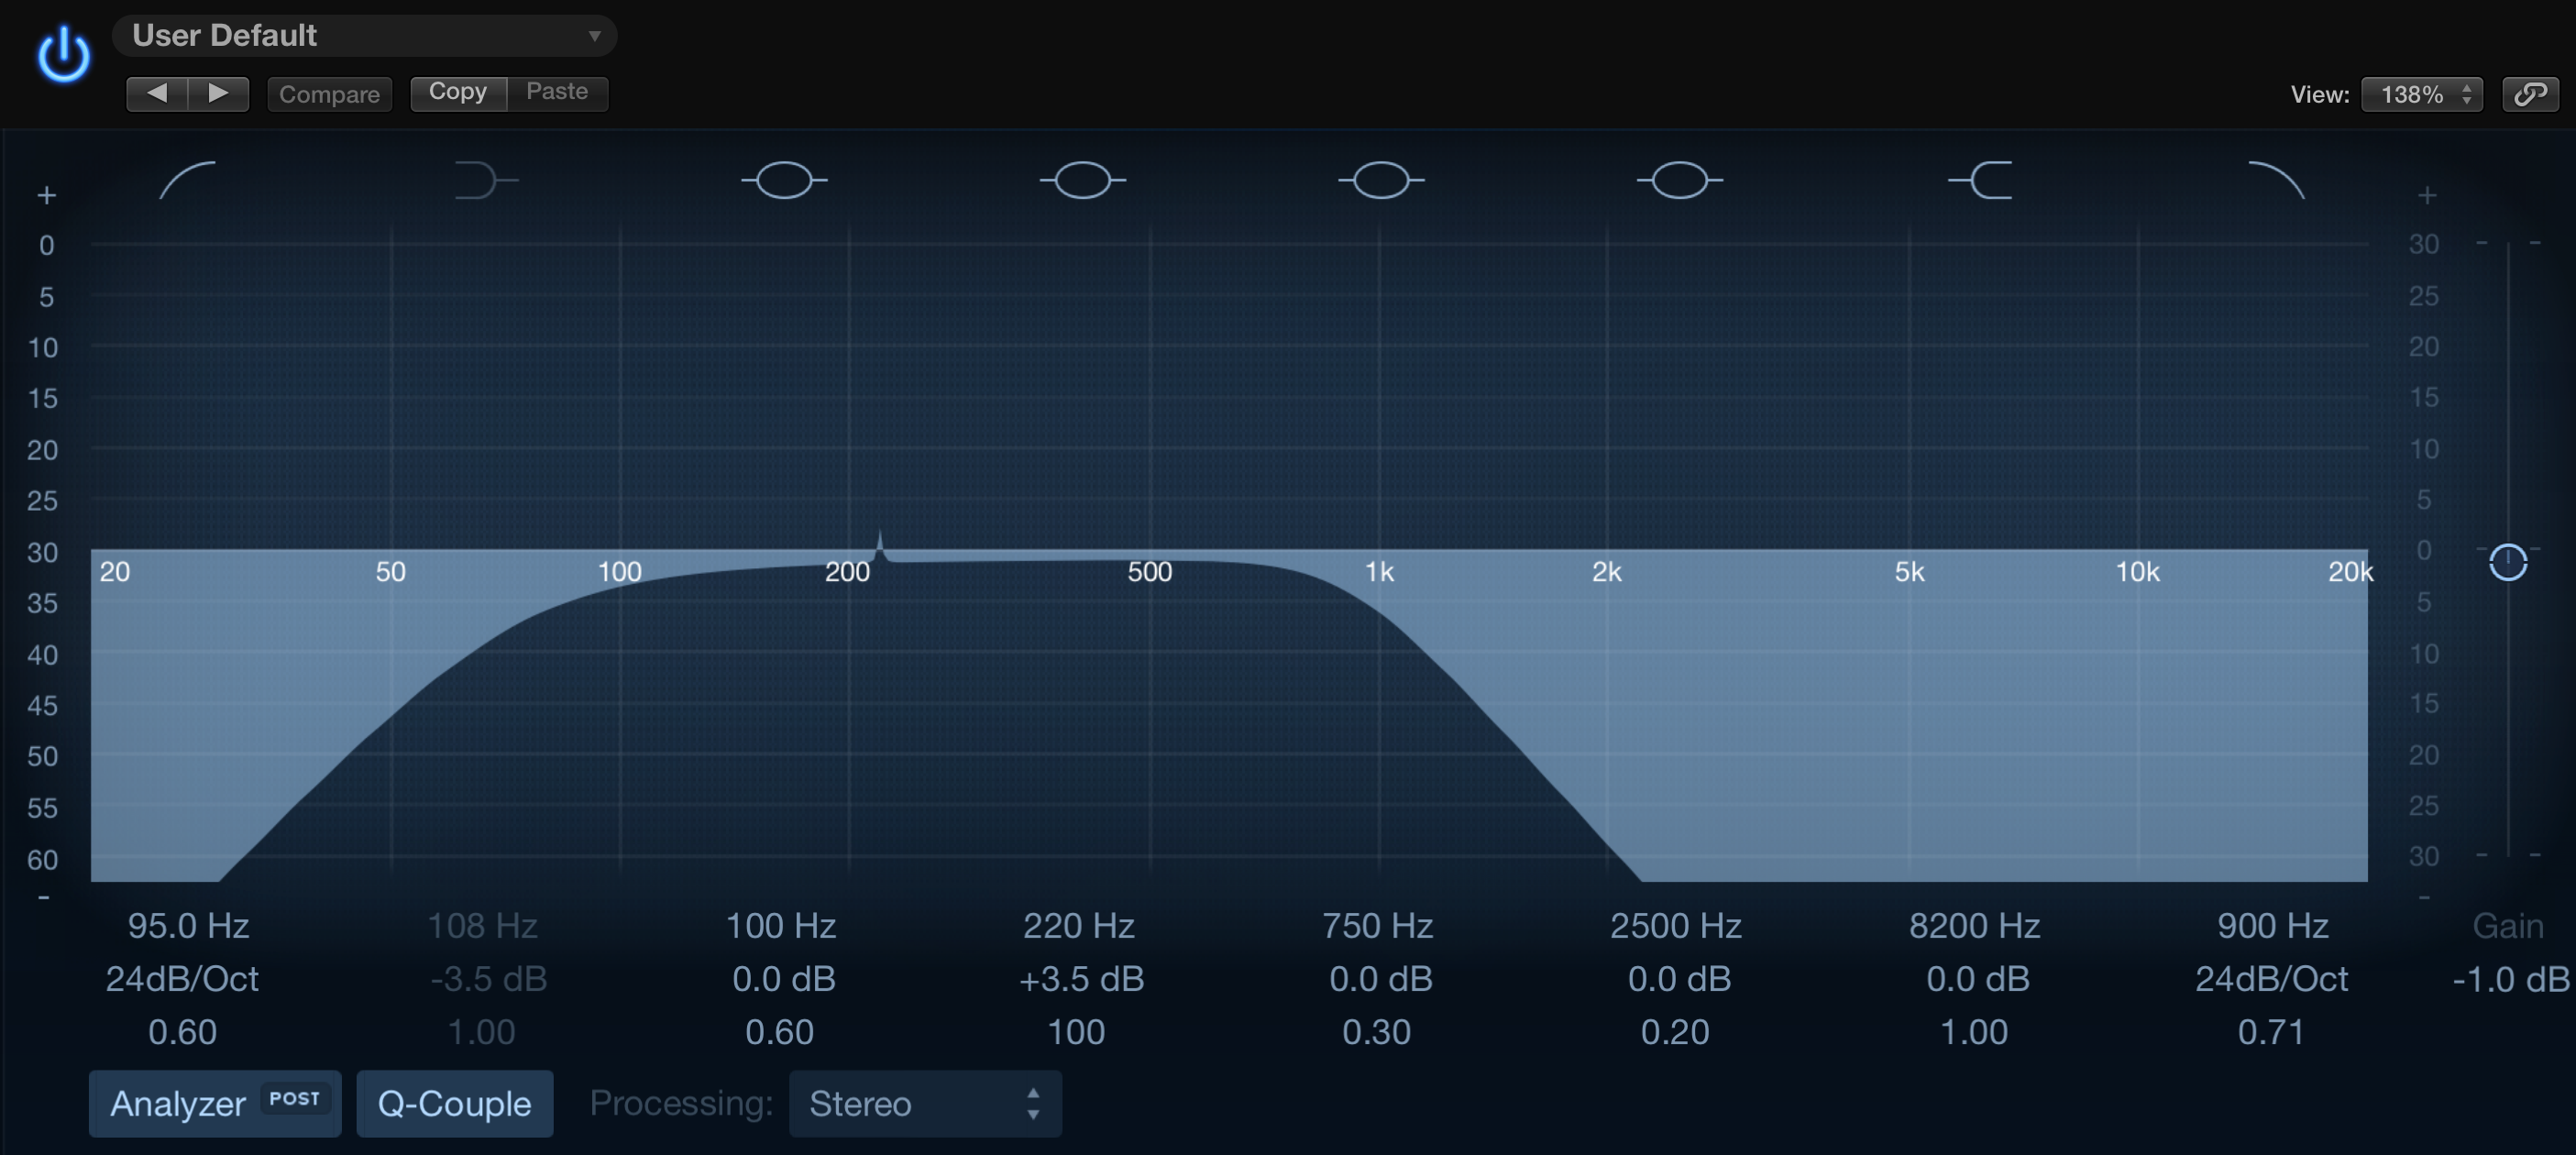
\includegraphics[width=\textwidth,height=0.25\textheight]{Modified_Click_EQ}}
    \label{fig:modClick}
\end{figure}

\textbf{A1b} and \textbf{A3b} however required a swing or legato type of chime in order to convey filling the interstitial space. To capture this effect the Klopfgeist tonality was increased to unity and tuned -27 semitones lower which served to both soften diminish the discrete click, provided an elongated or continuous audible sensation. 

To give the impression of a sound that was ramping up in amplitude and decaying after the peak, a tremolo effect which mimics a sawtooth wave was added to the signal chain as seen in Figure \ref{fig:modClick}. 

Last, a multi-band EQ was placed at the end of the signal chain with a bandpass filter from 95Hz-750Hz removing any unwanted frequency presence with a 3.5dB high-Q peak at 220Hz to emphasize the tonality.

The resultant waveform encapsulated the occupation of the interstitial space. A comparison of this waveform in contrast to it's discrete counterpart is shown in \ref{fig:click_comparison}. Note the envelope of signal (b) follows a natural build up and decay.

\begin{figure}[H]
    \centering
    \caption{Metronomic waveform comparison}
        \subfloat[A3a1: discrete audible click]{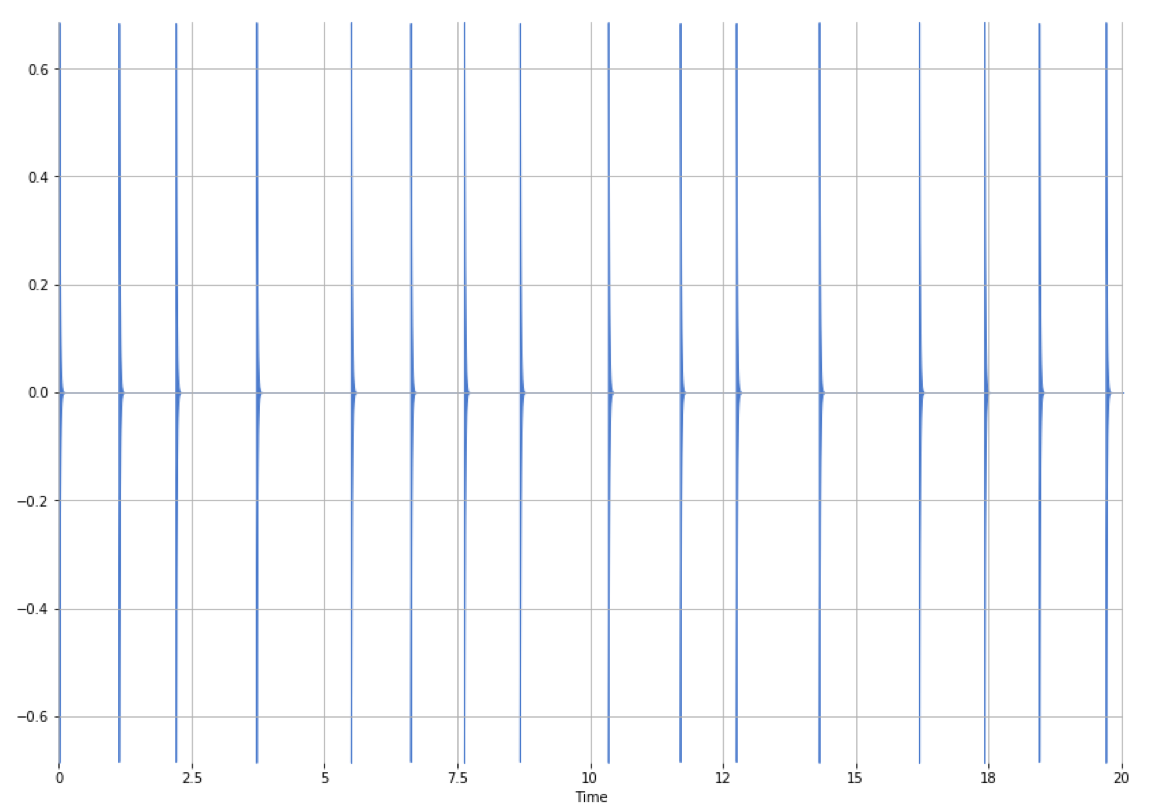
\includegraphics[width=0.5\columnwidth]{Click_waveform}}
        \subfloat[A3b1: interstitial tone]{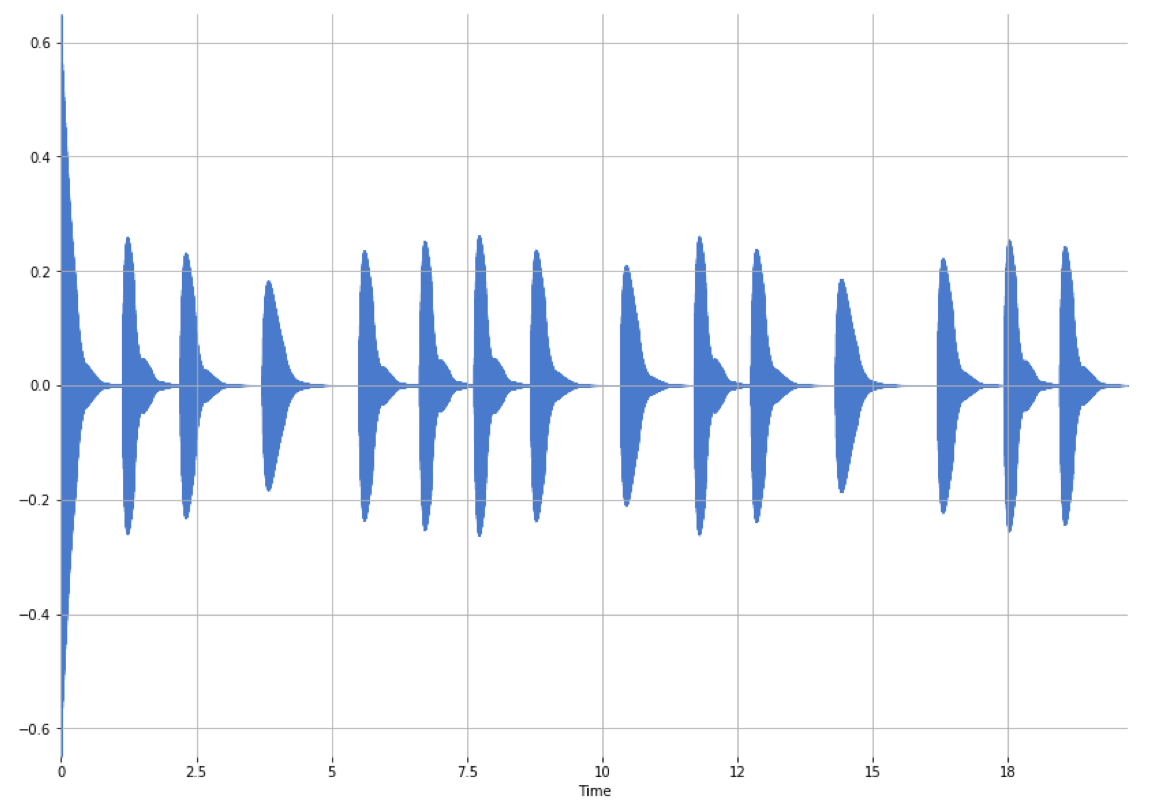
\includegraphics[width=0.5\columnwidth]{SwingClick_waveform}}
    \label{fig:click_comparison}
\end{figure}

\subsubsection{Stacatto and legato melody}
As a specific musical listening task, test cases \textbf{A2a}, \textbf{A4a} and \textbf{A2b}, \textbf{A4b} involve synchronization to a simple melodic sequence of notes. The music chosen was the nursery rhyme \textit{Pat-A-Cake}. The initial mockup was drafted in Sibelius and exported to Logic Pro X for bpm adjustment.

Each quarter note represents a beat and therefore a 1:1 synchronization tap onset task. In order to emphasize a discrete event for test cases \textbf{A2a} and \textbf{A4a}, notes were input as stacatto, shown below in Figure \ref{fig:patacakea2a}.

\begin{figure}[H]
    \centering
    \includegraphics[width=\textwidth]{Pat-a-Cake_a2a}
    \label{fig:patacakea2a}
\end{figure}

The interstitial counterparts (\textbf{A2b}, \textbf{A4b}) similarly underwent crescendo and decrescendo after every note onset with forte accents surrounded by mezzopiano to give the impression of amplitude build up and decay, shown below: \ref{fig:pat-a-cake_a2b} 

\begin{figure}[H]
    \centering
    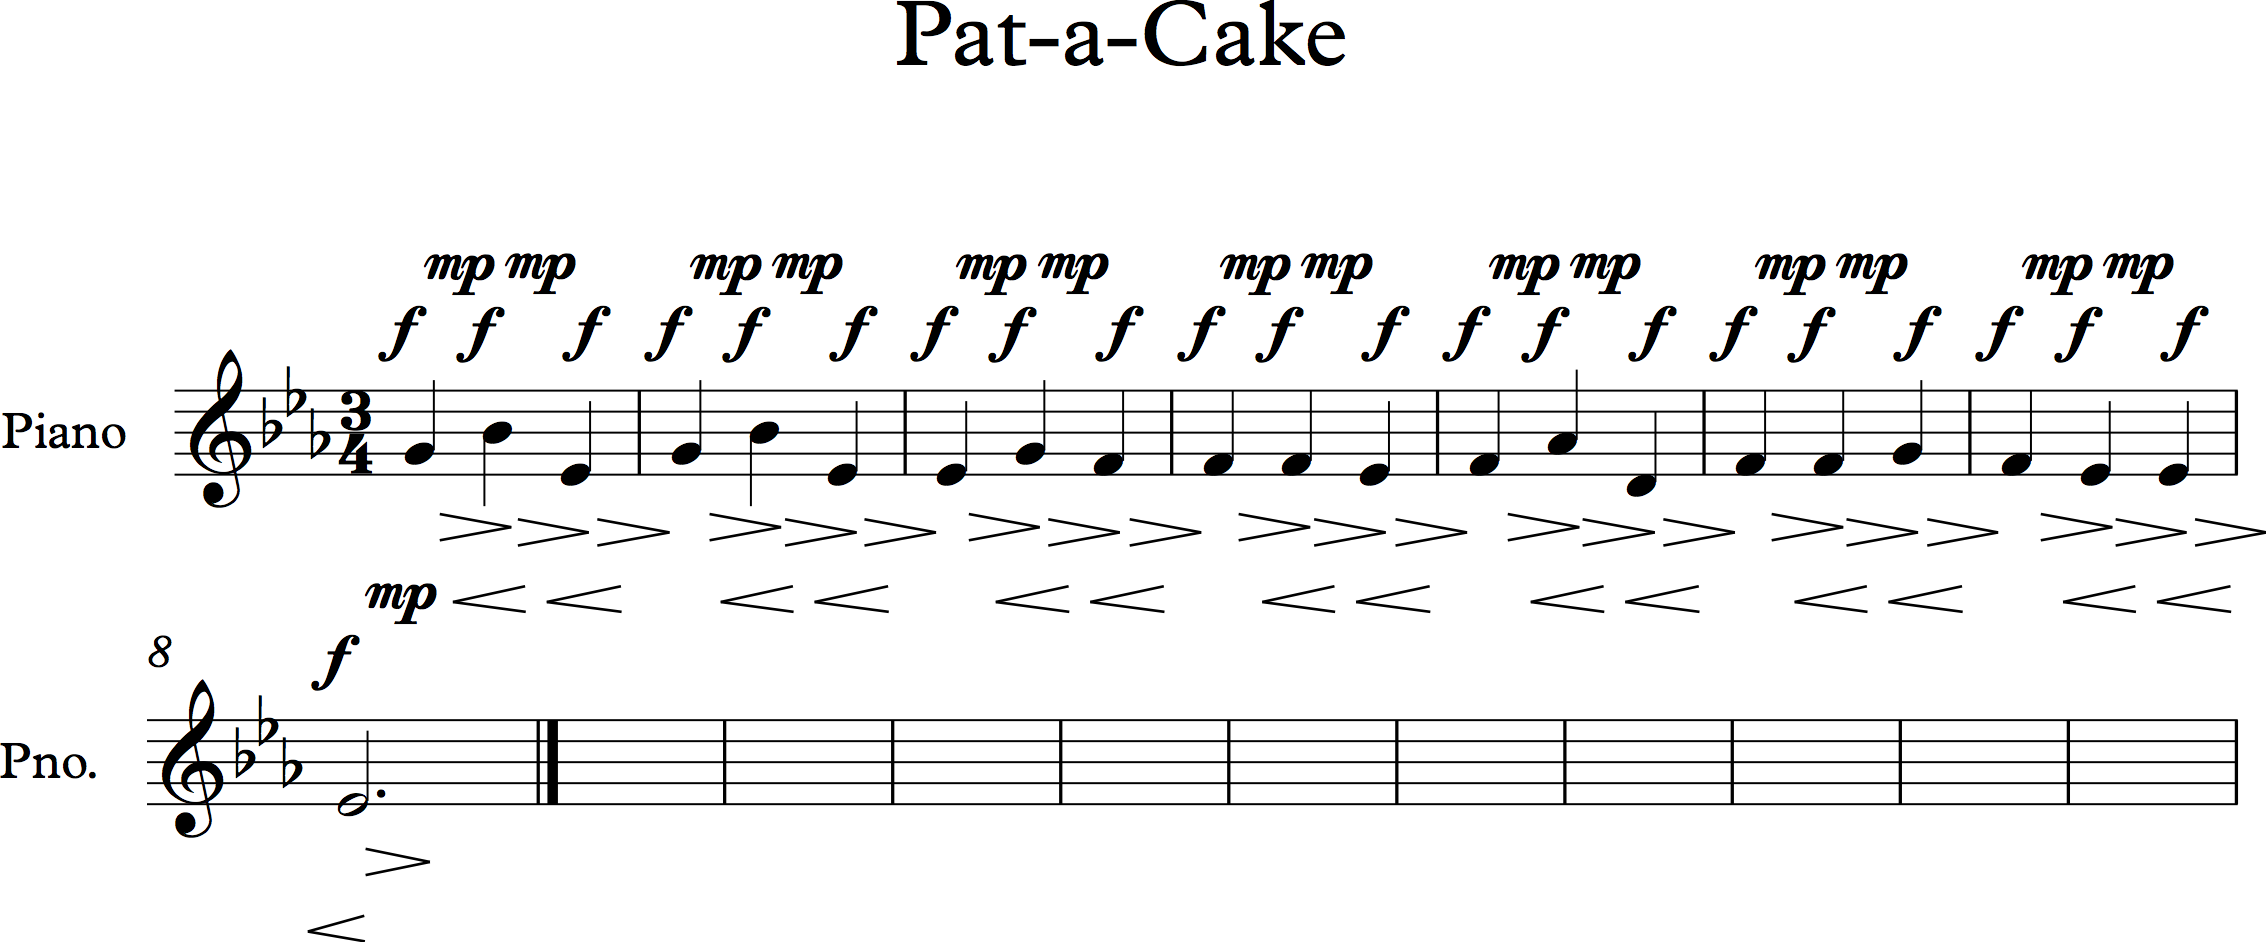
\includegraphics[width=\textwidth]{Pat-a-Cake_A2b}
    \label{fig:pat-a-cake_a2b}
\end{figure}

Note below in Figure \ref{fig:music_comparison} the gradual, nearly exponential decay displayed in the interstitial tone as a result of the legato input along with the amplitude difference due to the forte accents.

\begin{figure}[H]
    \centering
    \caption{Musical waveform comparison}
        \subfloat[A2a1: stacatto melody]{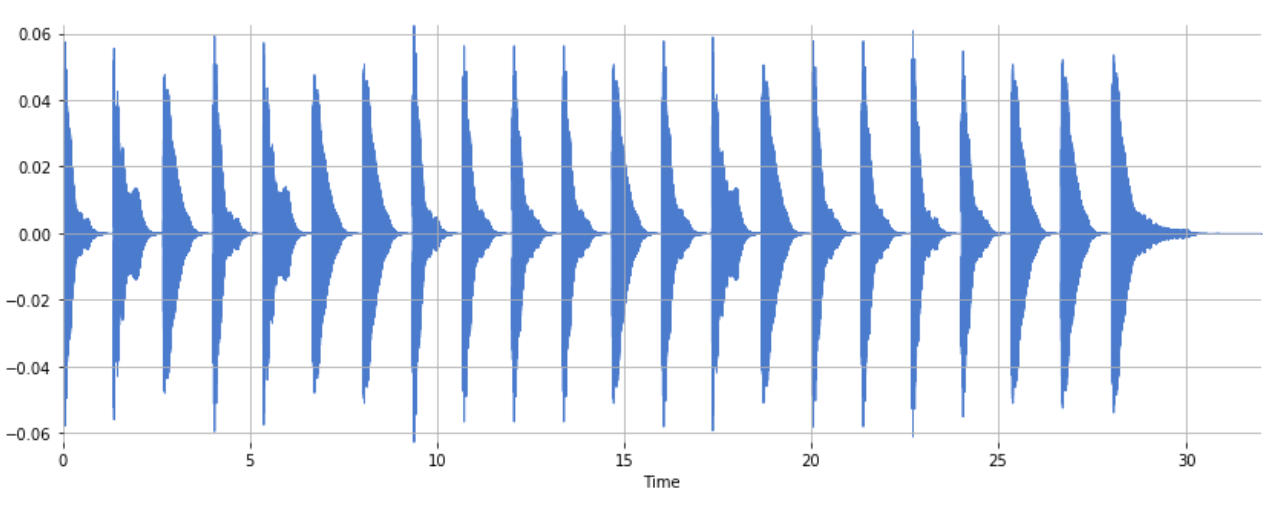
\includegraphics[width=\columnwidth]{A2a1_waveform}}
        \qquad
        \subfloat[A2b1: legato melody]{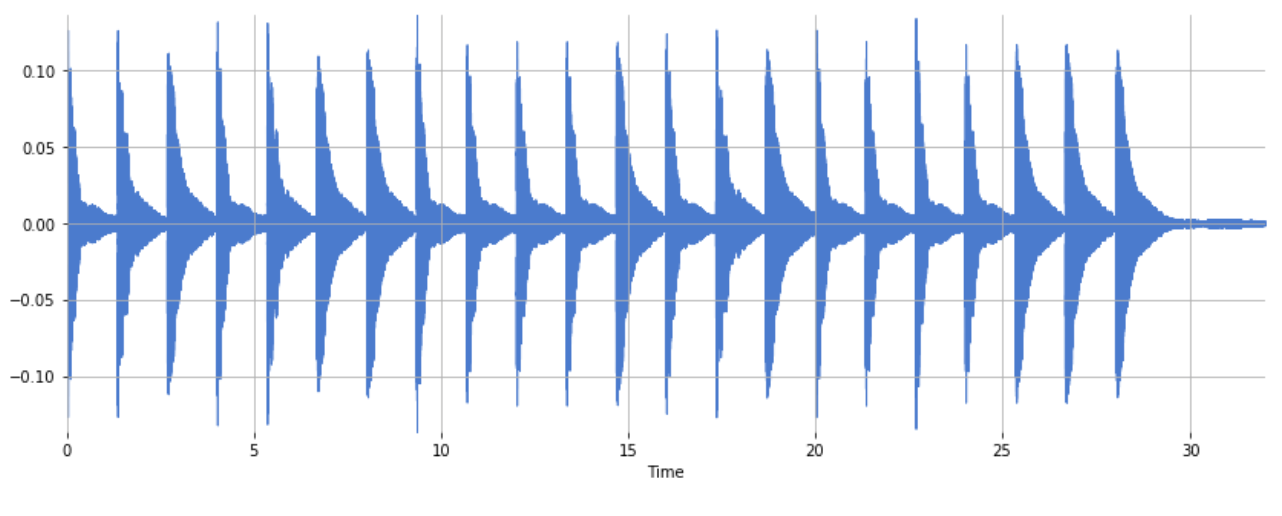
\includegraphics[width=\columnwidth]{A2b1_waveform}}
    \label{fig:music_comparison}
\end{figure}

\subsubsection{Dynamic tempi manipulation - audio}
Dynamic manipulation of tempo was accomplished in \textit{Logic Pro X} through automation of the tempo parameter over the time period of the desired waveform. Each test case started on one of the pre-defined BPM's (45, 90, 135, 180) but traversed either sinusoidally or triangularly through segmented time blocks as peaks and troughs ranging plus or minus 15 bpm; shown in \ref{fig:dynamic_audio}.

\begin{figure}[H]
    \centering
    \caption{Dynamic audio tempo automation patterns}
        \subfloat[45 +/- 15]{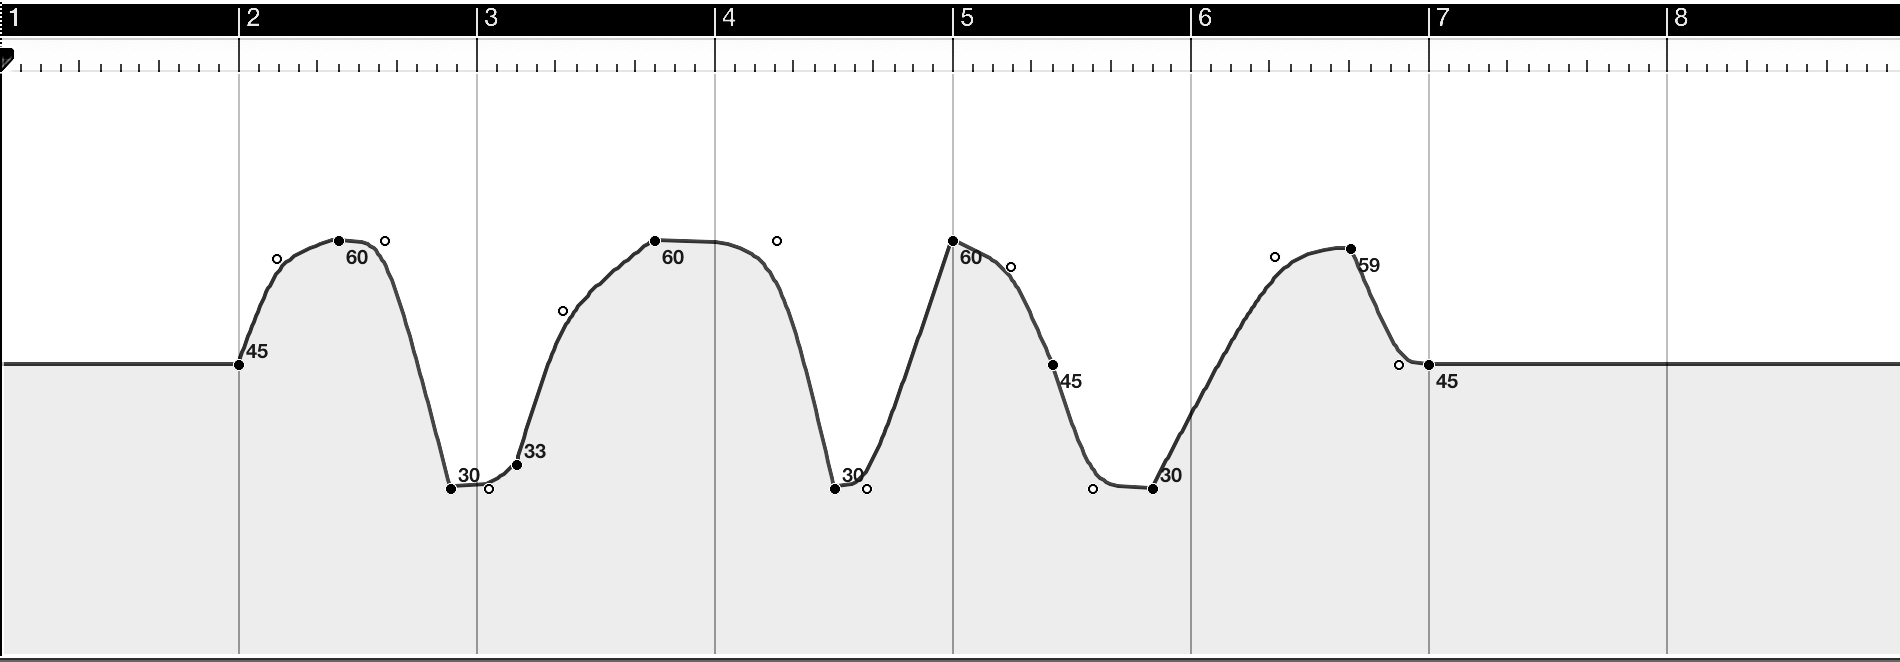
\includegraphics[width=.5\columnwidth]{dynamic_45}}
        \subfloat[90 +/- 15]{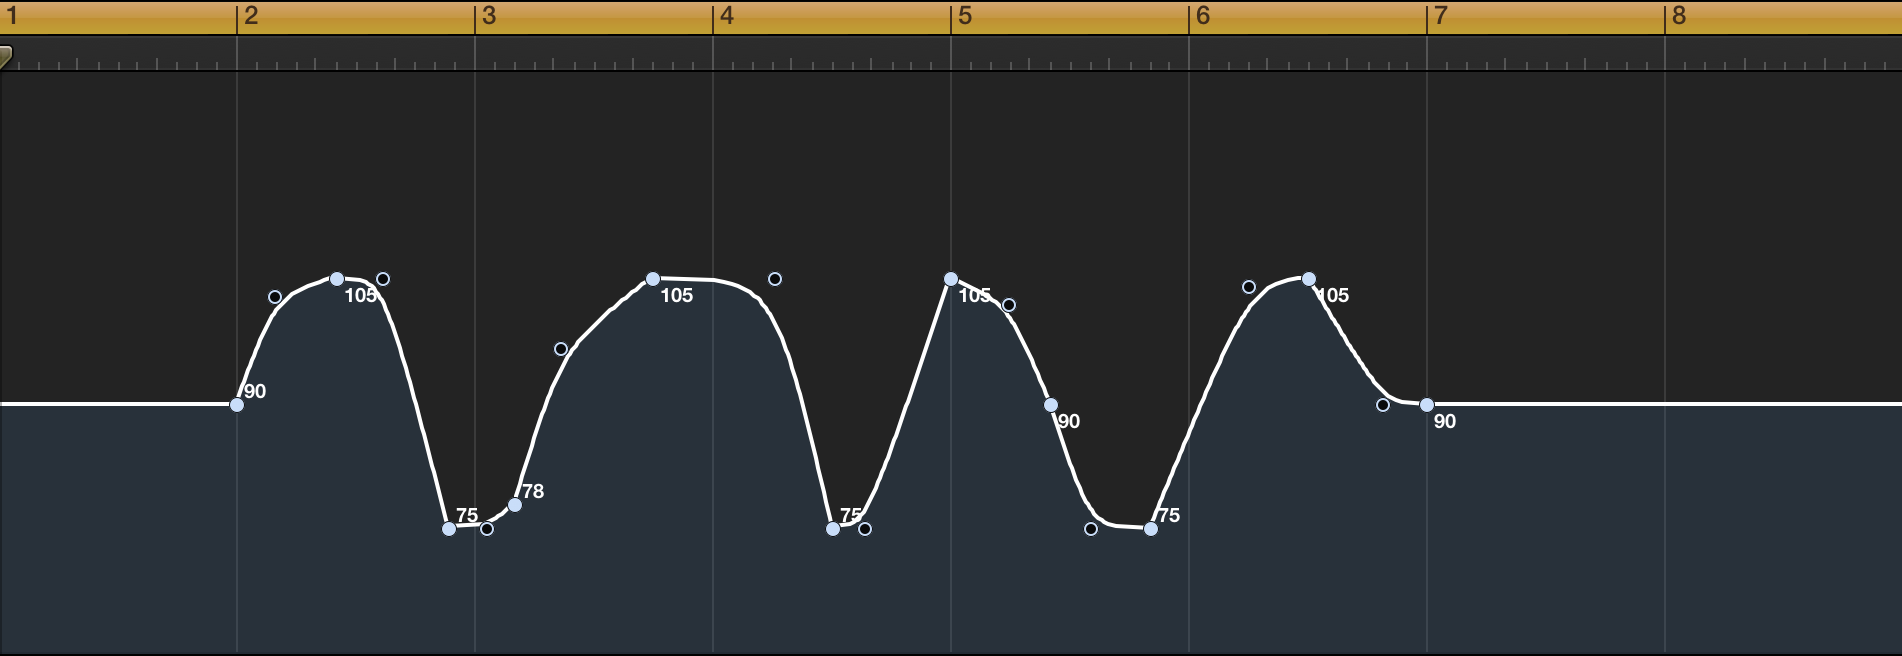
\includegraphics[width=.5\columnwidth]{dynamic_90}}
        \qquad
        \subfloat[135 +/- 15]{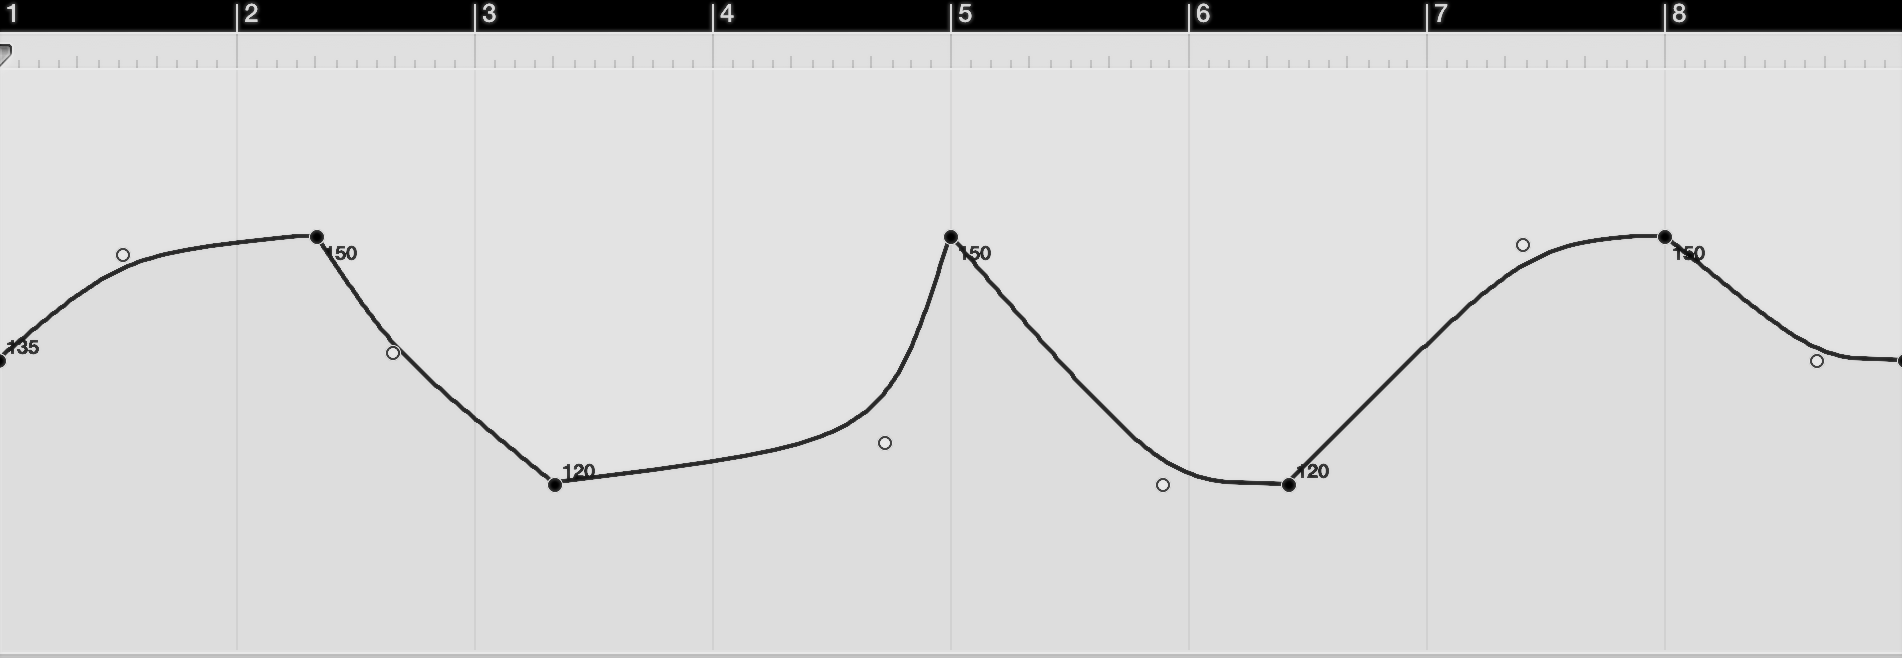
\includegraphics[width=.5\columnwidth]{dynamic_135}}
        \subfloat[180 +/- 15]{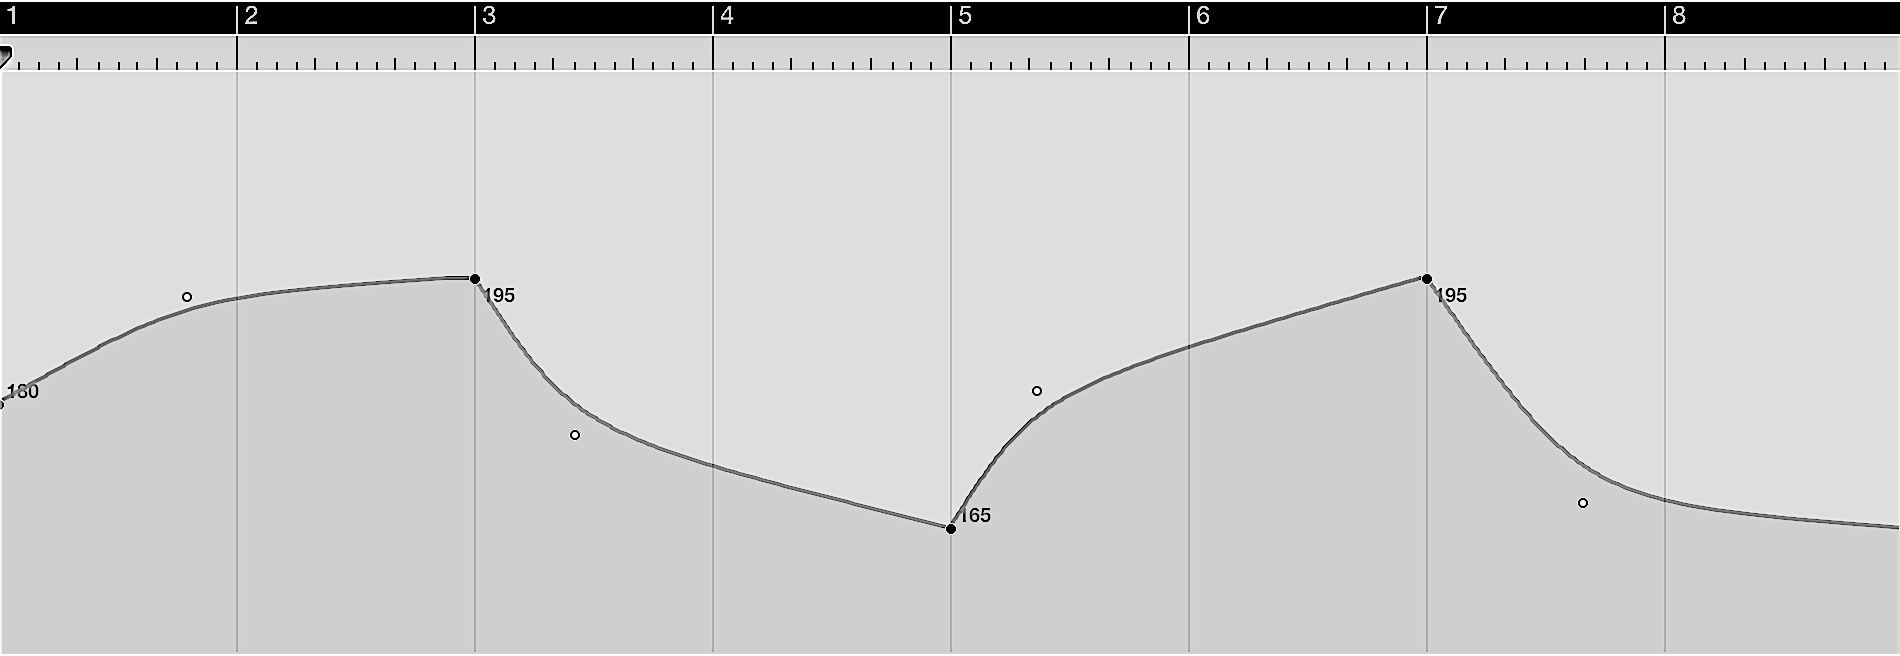
\includegraphics[width=.5\columnwidth]{dynamic_180}}
    \label{fig:dynamic_audio}
\end{figure}

\section{Test Suite}
High precision data acquisition and the minimization of delay were the central foci of the test suite design. Due to the extensive amount of publicly available libraries, multithreading capability, pandas dataframe structure, and plot integration via matplotlib, \textit{Python} was chosen as the development environment. Complementary to the software platform was the implementation of a tap onset detection mechanism via force sensitive resistor (FSR) on the \textit{Arduino Uno}. 

\subsection{Software Development} \label{development}
A pseudocode breakdown of the framework is provided below. The methods were written in Python in object oriented fashion. The critical sub-components of the test suite are discussed below. 

\subsubsection{GUI}
The GUI was written with the Tk framework\footnote{\url{https://en.wikipedia.org/wiki/Tk_(software)}}. It consisted of three frames and a main class which instantiated the others. The \textit{StartPage} stored the \textit{userName} to be later anonymized via a simple char to int summary conversion technique. The next click presented the user with the \textit{InstructionPage}. Once accepting of the terms of the test, the final \textit{TestPage} readies the user for the upcoming practice tests and triggers the main code execution once the \textbf{Start Test} button is pressed.
\subsubsection{Multithreading}
Since the test suite read from two serial devices simultaneously, there needed to be a non-blocking methodology that allowed uninterrupted flow control; this was provided from the import of \textit{threading} from the \textit{Thread} library. Once the user started the test, the practice mode began. Here a thread was initiated which created the beep timer. At the end of the audible tone the thread completed and a second thread started passing the arguments of the test cases (either Haptic or Audio) into the method. A third thread was started simultaneously to the second which focussed on getting the tap onsets. These threads worked in parallel during the test case duration and upon completion incremented a counter and passed argument to the data analysis method for logging.
\subsubsection{Haptic Onset Detection}
The haptic test cases were broken down into dictionary lists containing arguments to be passed to the \textit{haptic} method. The arguments were dependent on the mode of operation the test case called for, the tempo desired, the time of execution, and whether the tempo was to change dynamically over time.

The mode and tempo are written over serial to the haptic device and a start time is recorded. From here the program enters a while loop for the duration of test execution reading in from serial while awaiting the "onset" message. Once received it appends to a list for later data logging.

If however, the test case calls for the dynamic mode of operation, the execution time is broken into quarters. Each quarter either increments or decrements the tempo based on the argument passed in by the test case. In this fashion, the dynamic haptic test cases closely emulate the sinusoidal tempo automation of the dynamic audio tests.
\subsubsection{Tap Onset Detection}
The tap method read from the incoming Arduino Uno serial line and decoded bytes from the buffer. The preamble was the char "B" which signified an incoming packet. The onset was timestamped and stored in a dataframe and this process repeated until either the haptic or audio methods passed through the closeFile global variable signifying the end of execution.
\subsubsection{Audio Onset Detection}
The wav files were individually analyzed using the \textit{librosa} package based on Steve Tjoa's MIR (Music Information Retrieval) website.\footnote{\url{https://musicinformationretrieval.com/onset_detection.html}}
The onsets were detected via librosa's onsetDetect method which computed the spectral novelty function to find the peaks. The computation was then converted from frames to seconds with nearly nanosecond precision (See Figure \label{fig:AudioOnset}). The onsets for each audio test case were then stored in dictionary lists to be called upon later by the test suite in order to add timestamps to the seconds stored in the list.
\begin{figure}[H]\ref{fig:AudioOnset}
    \centering
    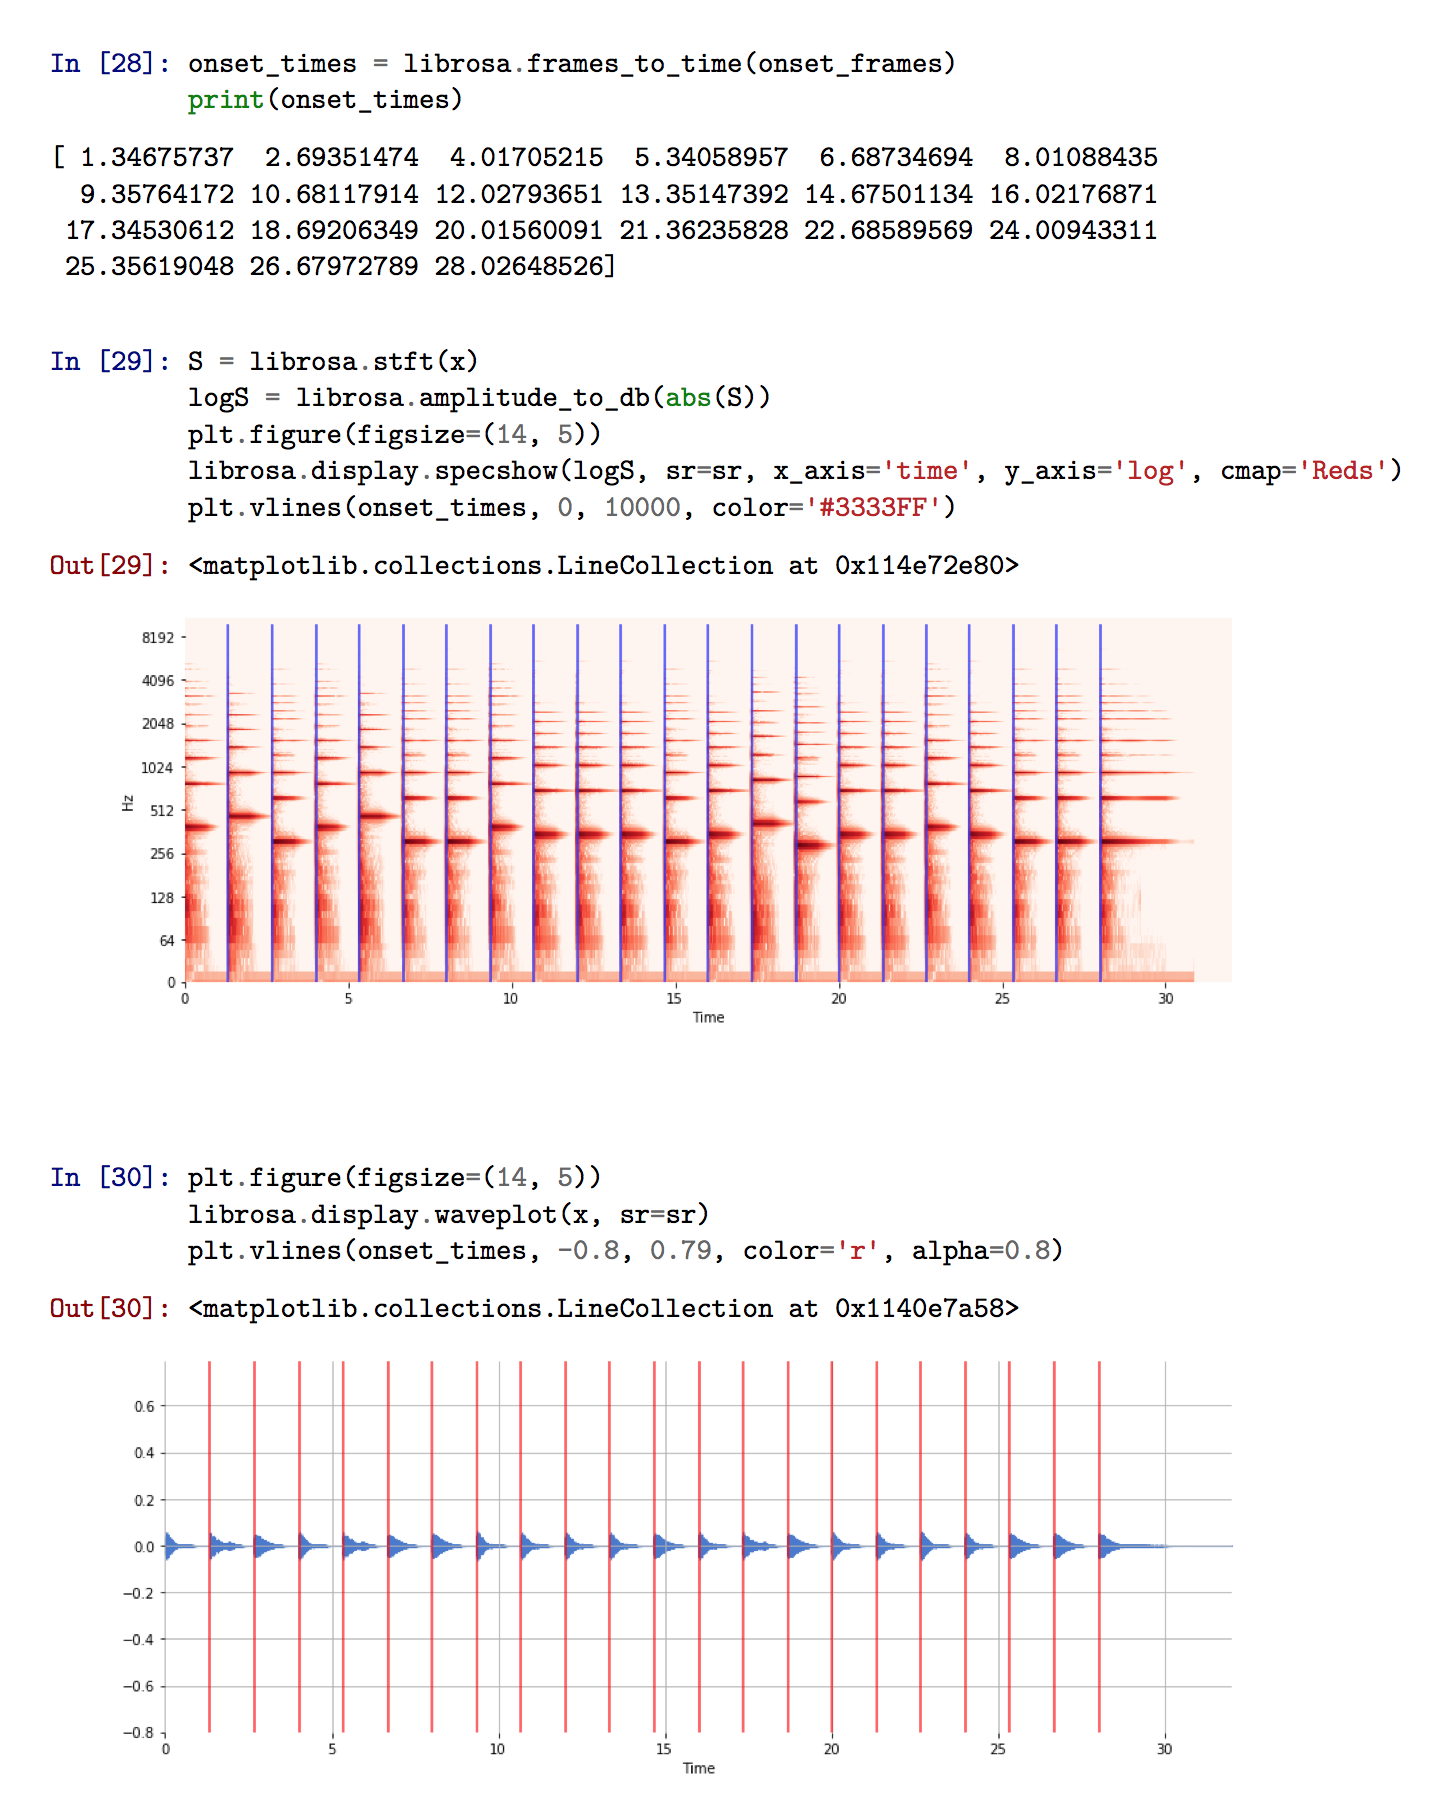
\includegraphics[width=\columnwidth]{audioOnset}
    \caption{Test Case A2a1 Audio Onset Detection Example}
\end{figure}
\subsubsection{Audio Rendering}
A mixer object was imported from \textit{pyGame}, a module for loading sound objects and controlling playback. The object was initialized at 16 bit 44.1 kHz over 2 channels with a buffer size of 64. The buffer size was experimented with to balance lowest latency without audio dropout. The playback method loaded the audio file passed through the method argument and set the volume. Once the mixer play method was called a separate \textit{getBusy} object ran in a while loop while the audio was played back to find out if the buffer was still busy or not. This object gathered the audio file playback start time which was appended to a temporary list to be added to the audio onset dictionary list aforementioned and written to a dataframe.
\subsubsection{Data Logging}
All of the timestamps and onsets were piped into a Pandas dataframe. Pandas is almost like an SQL table and allows for mutable size, different column types, manipulation of axes, arithmetic operations, and easy plotting. Duplicate entries recorded were dropped for same measure along with the first and last values of each test to ensure fairness. From the tap and true onsets, the asynchrony was calculated and stored in milliseconds. From the difference between the current line and next line true onset, the inter onset interval (IOI) was recorded and output in milliseconds. Missed taps were tallied based on null values for tap onsets where true onsets existed. Last, the phase correction response was gleaned as the delta between current and next asynchrony.
\subsubsection{Sanitization Procedure}\ref{sanitizationProcedure}
It was important to have a method in place for synchronizing results if the user ever missed a tap and tried to get back on beat. Without it, there would be an undesired shift and the asynchrony values would be unrealistically high. The numpy select method was utilized to filter choices based on conditions within an array (or dataframe). A max point of acceptance was established by taking half the IOI added to the true onset. Similarly the mix was taken as half the prior IOI added to the true onset. Every tap onset within a test cases dataframe was shifted through the max and min thresholds to determine whether a tap onset belonged to a different true onset. The new column created was called the \textit{Sanitized Tap Onset} and from here the \textit{Sanitized Asynchrony} was calculated.
\subsubsection{Plotting}
At the end of the data analysis method a plot based on the current dataframe test case was presented using plotly\footnote{\url{https://plot.ly/}}. This was a snapshot of the time vs. onset and can be seen in Figure \ref{fig:TestCaseFeedbackEx}.
\subsection{Tap Test Hardware} \label{tap_arduino}
Closely following the design outlined in \ref{schultz2016tap}, a force sensitive resistor was connected across 5 V and the analog input pin A0 of the Arduino Uno. Bridged between A0 and GND was a 10 K resistor acting as a resistive divider. The code was based on the \textit{$fsr_silent_disc.ino$} developed by Schultz but expanded and modified to better suit this project. 

\begin{figure}[H]
    \centering
    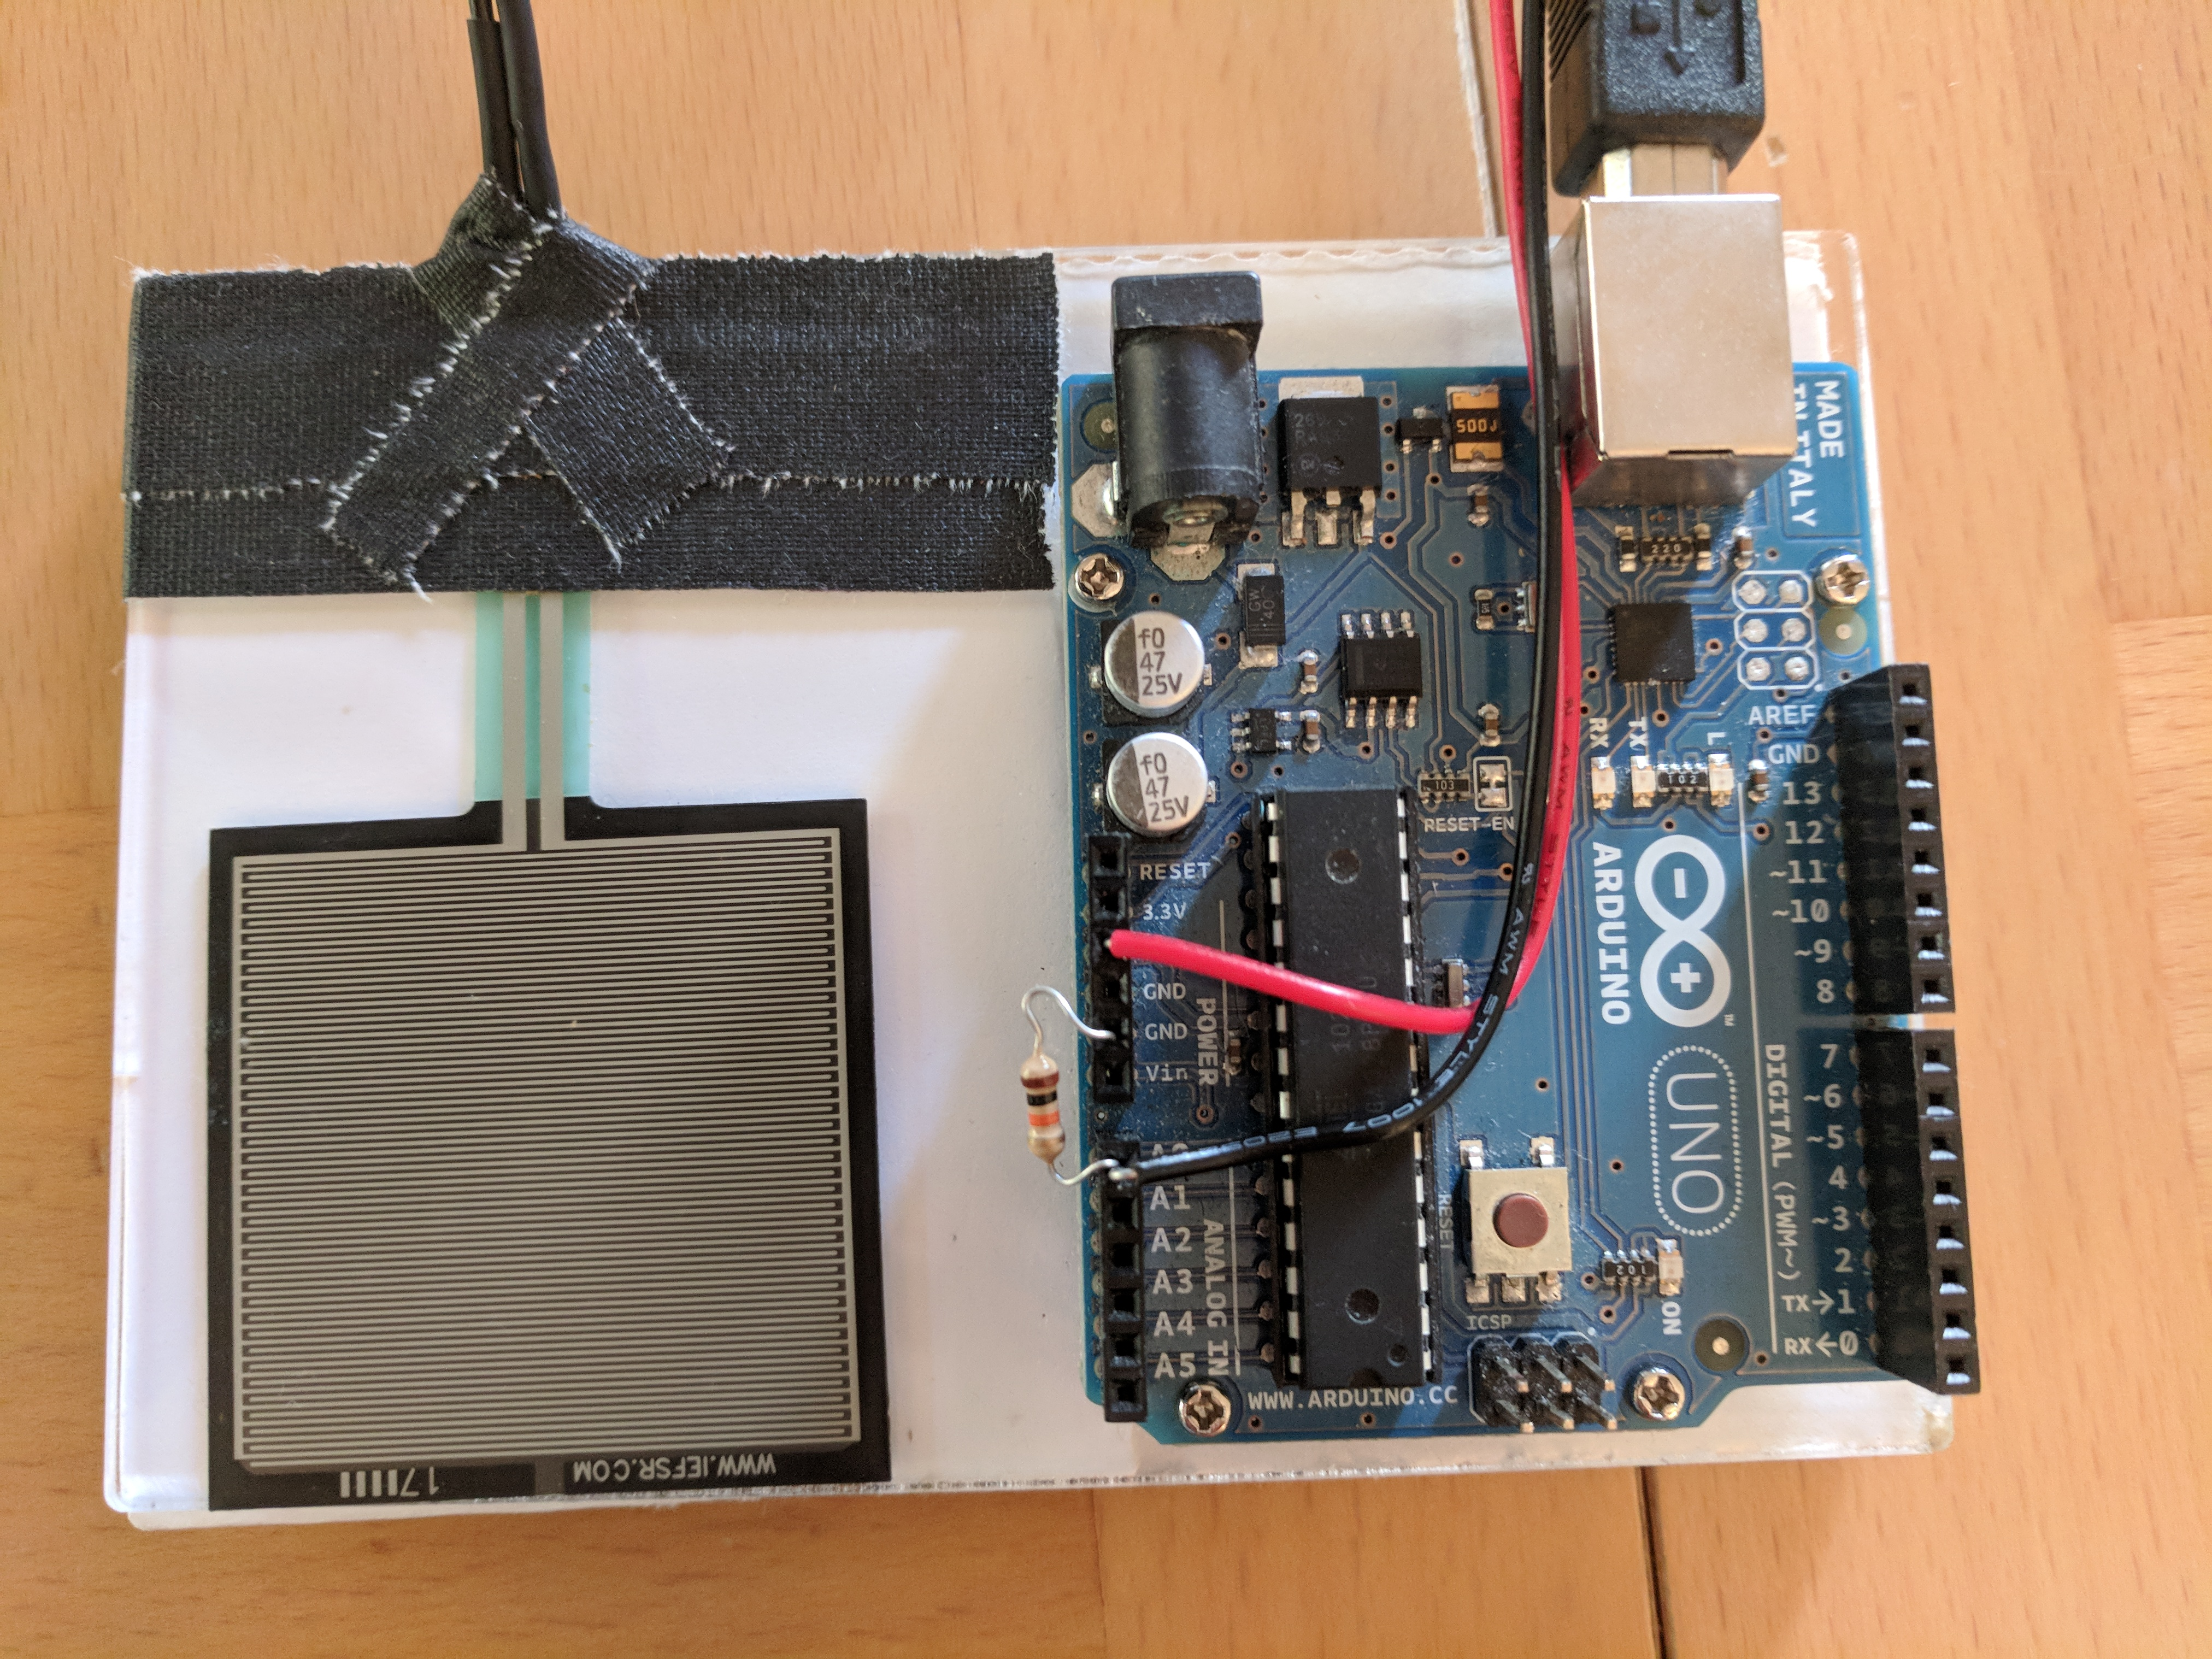
\includegraphics[width=\columnwidth]{FSRHW}
    \caption{Arduino Tap Test Hardware}
\end{figure}

Schultz had defined thresholds to determine the minimum FSR tap necessary to classify as a response. If the analog reading exceeded the threshold then the tap was windowed further to prevent debounce and the data packet readied for transmission. The packet consisted of the character "B" followed by onset time, offset time, and max force from the FSR reading, ending with the character "E" to signify the end of the packet. The trade off between responsiveness and threshold required to prevent a double bounce was finely tuned via oscilloscope and will be further explained in Section \ref{FSRregistry}.

\subsection{Setup} \label{testSetup}
To initialize setup, the subject is seated and given a pair of closed-back headphones. The FSR is situated to their preference, either dominant or non-dominant hand, and secured into place. Unlike a keyboard or button the FSR gives little to no feedback or rebound. This ensures a confident tap on each onset while providing no tactile response. The approach seeks to avoid intrinsic lag due to its independence of mechanical components. The delay limit is defined by the threshold applied in the software to avoid debounce, as discussed in Section \ref{development}

\begin{figure}[H]
    \centering
    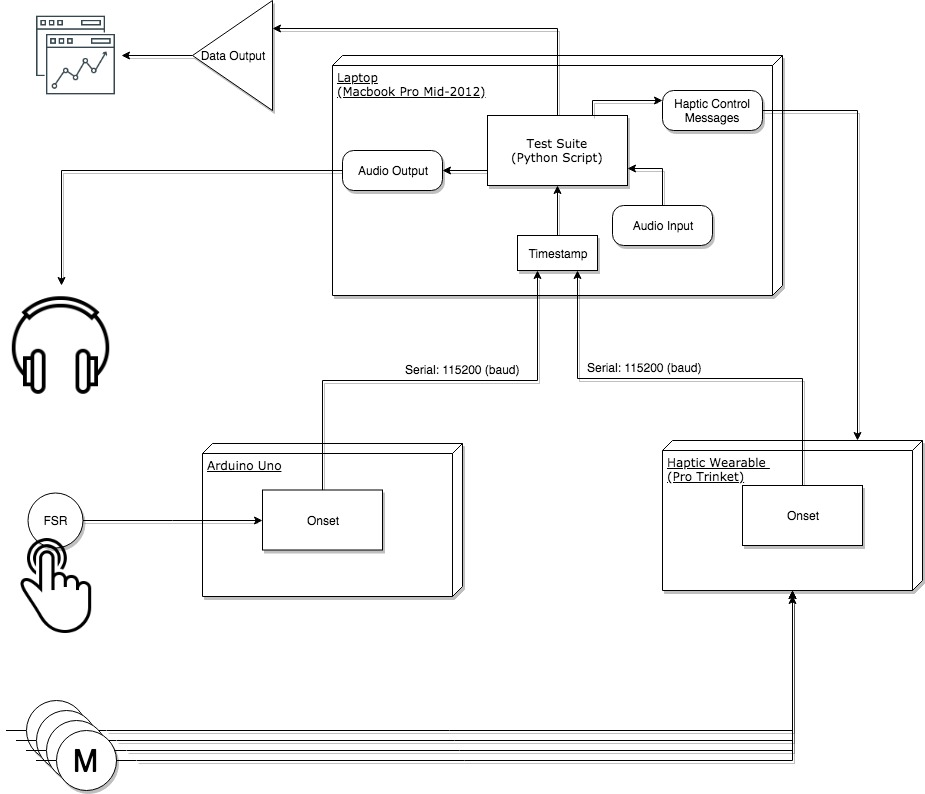
\includegraphics[width=\columnwidth]{TestSuiteFlowDiagram}
    \caption{Test Suite Flow Chart}
    \label{fig:TestSuiteFlowDiagram}
\end{figure}

The Python file \textit{testSuite.py} is run and the UI will prompt the subject to input their name, read the instructions, agree to the conditions of the test suite, and commence with the test. The first 8 are practice tests to get used to the haptic sensation as well as the variety of audible test cases. The order of test case execution is scrambled with a static seed pseudo-random generator such that every user encounters the same test order. Every iteration of the test plots the Tap Onset, True Onset, and Sanitized Onset  for the purposes of feedback and affirmation of correct tapping as seen in Figure \ref{fig:TestCaseFeedbackEx}. Upon completion of the 48 test cases, the users are asked to fill out a survey for feedback.

\begin{figure}[]
    \centering
    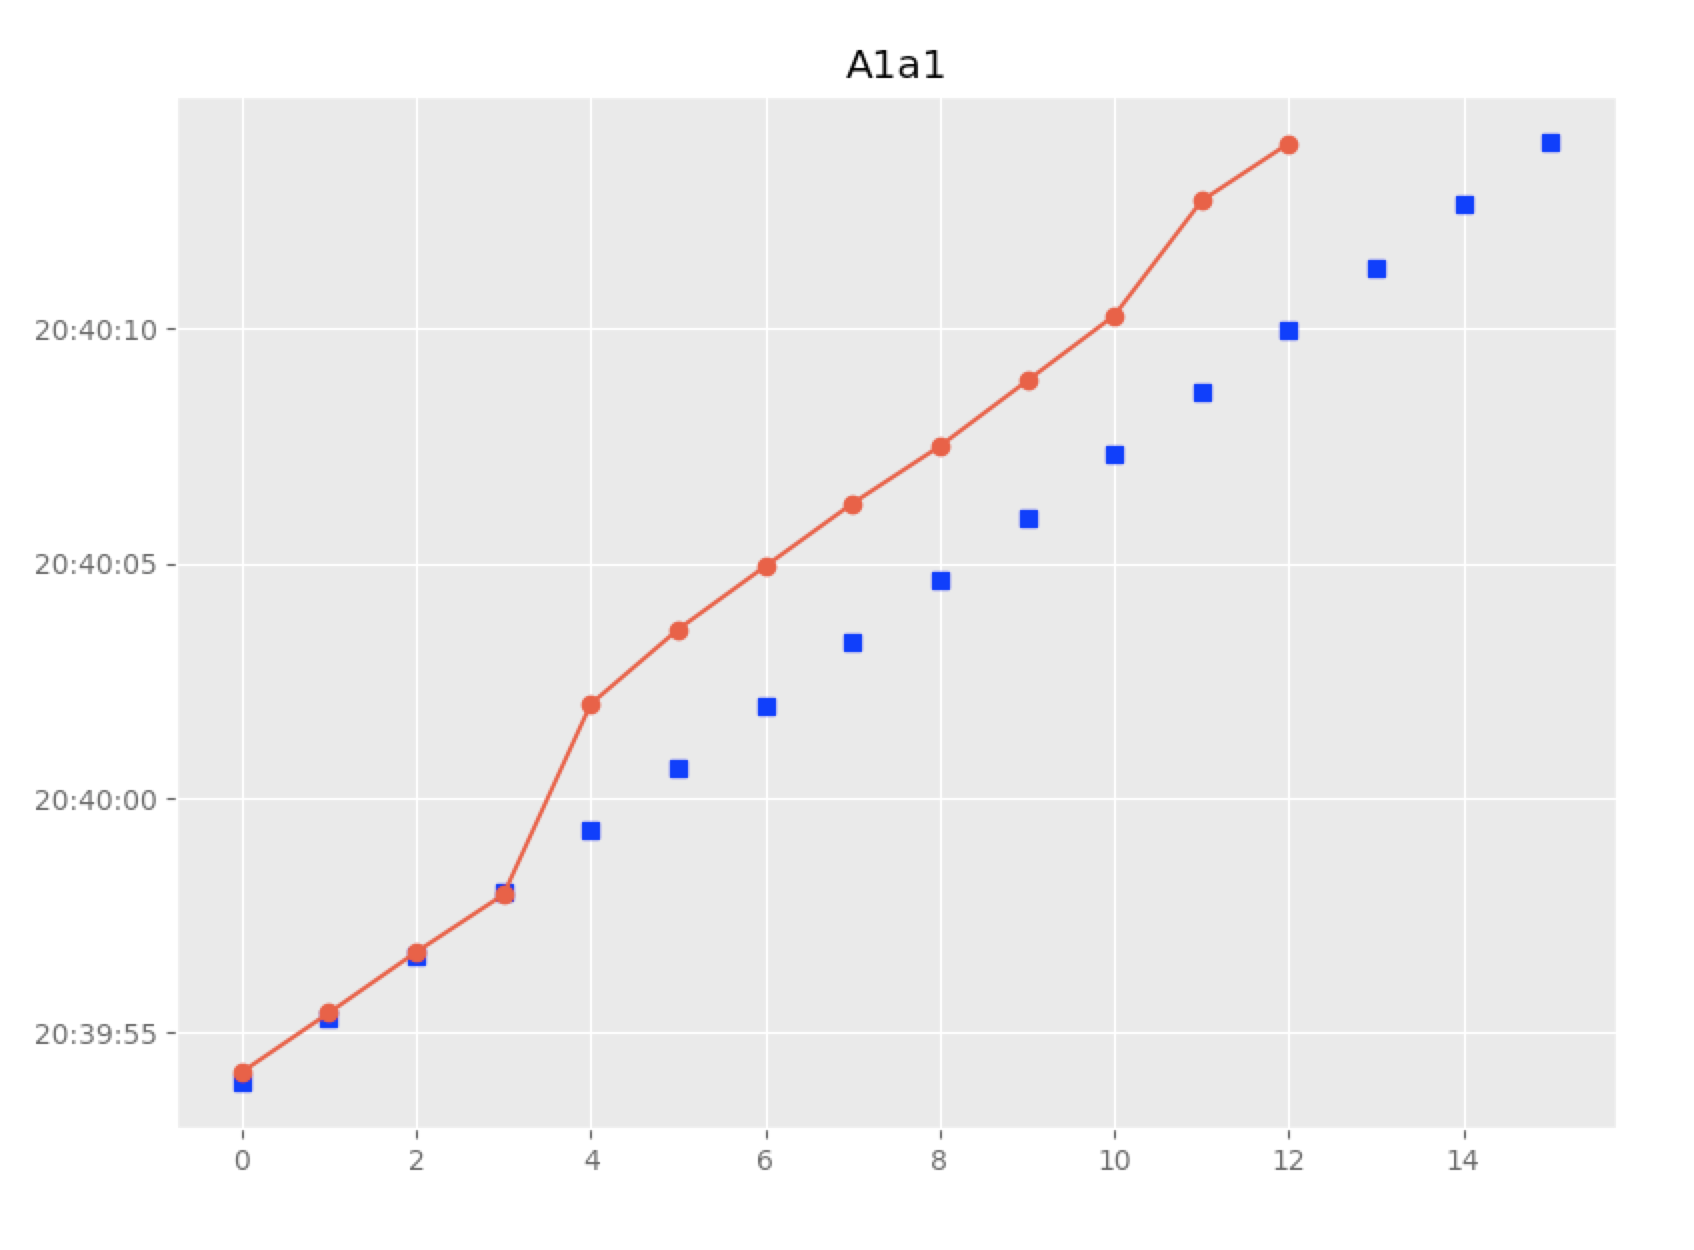
\includegraphics[width=\columnwidth]{TestCaseFeedbackExample}
    \caption{Test Case Feedback Example: Red circles are the tap onset, blue squares are the true onset. The x-axis is the tap count, the y-axis is elapsed time.}
    \label{fig:TestCaseFeedbackEx}
\end{figure}

\subsection{Latency Evaluation} \label{latencyCalc}
Significant efforts were made to determine the overall latency of the test system and instill a level of confidence in the validity and accuracy of the data points acquired. The sources of potential latency were isolated into the components identified below.
\begin{itemize}
    \item FTDI-USB communication from Pro Trinket (16 MHz) to laptop
    \begin{itemize}
        \item According to section 3.1 of the datasheet for FTDI based chipsets\footnote{\url{http://www.ftdichip.com/Support/Documents/AppNotes/AN232B-04_DataLatencyFlow.pdf}} , FTDI USB-Serial communication to PC exhibits by default a round trip delay of 16 ms intrinsic to the packet scheduler. When the latency timer expires and the buffer is not yet full any data in the 62 byte buffer is sent along with a short 2 byte status message (total of 64 bytes).
        \item This 16 ms spec was confirmed by measuring incoming "onset" messages from the Pro Trinket over FTDI and comparing it to the known period. The jitter measurement was calculated and averaged via a custom script written in \textit{Go} and was found to average 8 ms in either direction, or a span of 16 ms. The swing seemed dependent on the period but always averaged to around 16 ms. See Figure \ref{fig:rtIndividual} for confirmation.
        \begin{figure}[H] \label{fig:rtIndividual}
            \centering  
            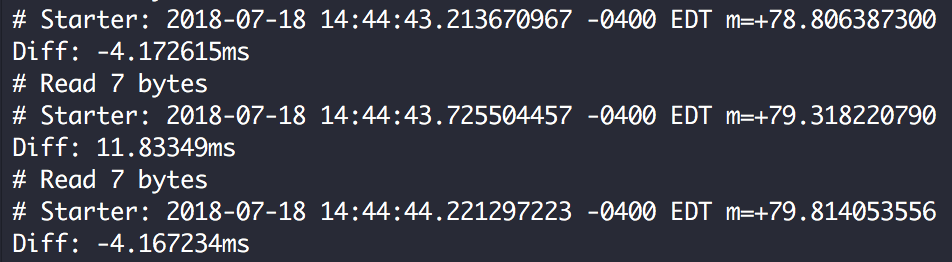
\includegraphics[width=\columnwidth]{rtIndividual}
            \caption{16 ms jitter on average for single device drift between "onset" message across FTDI over a set period of 500 ms}
        \end{figure}
    \item Serial round trip latency (TX Jitter)
        \begin{itemize}
            \item The round trip latency of a single packet containing the "onset" trigger was sent across a digital pin on the Trinket over to a digital pin on the Arduino Uno, which triggered it's own serial "onset" trigger message.
            \item The implications of this isolate the USB protocol scheduler as the main culprit for the latency seen during the test.
        \end{itemize}
    \end{itemize}
    \item The time to actually send the "onset" message across serial was a negligible 0.6 ms as shown in Figure \ref{fig:onsetMessage}
    \begin{figure}[H] \label{fig:onsetMessage}
        \centering
        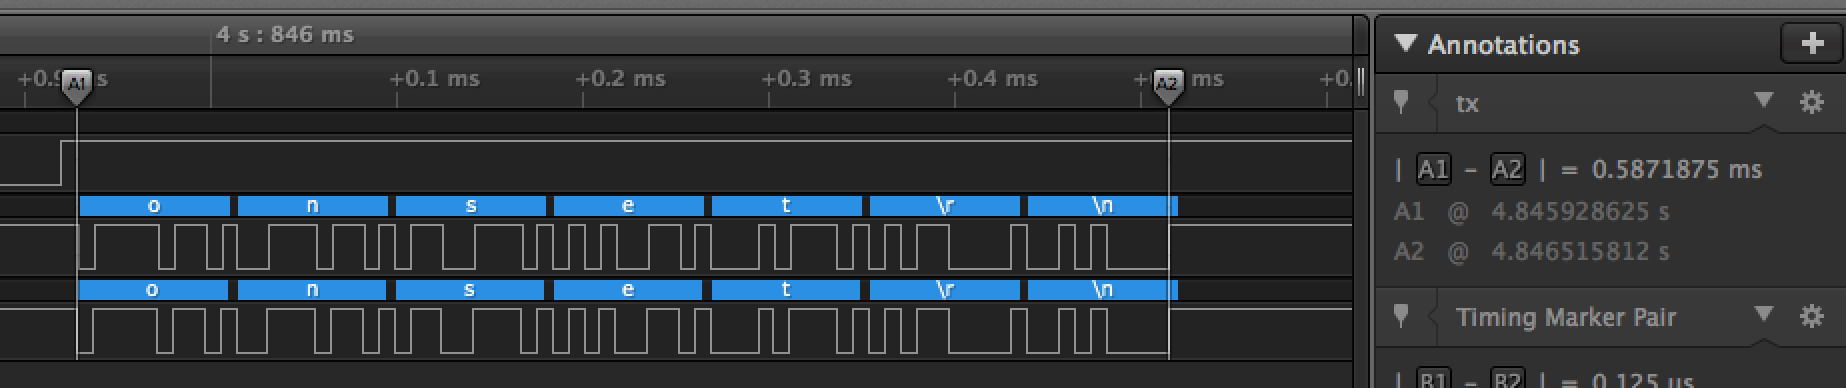
\includegraphics[width=\columnwidth]{onset}
        \caption{From the top: 1000 ms starter signal from Pro Trinket. Middle: starter TX line, End: stopper TX line on Arduino Uno}
    \end{figure}
    \item Time from FSR tap registry to Arduino TX \label{FSRregistry}
    \begin{itemize}
        \item Human input is never perfect. The tap onset needed to be triggered above the noise floor just enough to get the input. It took a few optimization runs to determine what constituted a real tap without triggering a second tap unintentionally. The original \textit{Tap Arduino} code would send the TX message only during the FSR ramp down or decay which introduced some latency. This bound was modified to instead be placed at the ramp up which minimized latency from tap to transmit to 294.4 microseconds as shown in Figure \ref{buttonTX}
        \begin{figure}[H]\label{buttonTX}
            \centering
            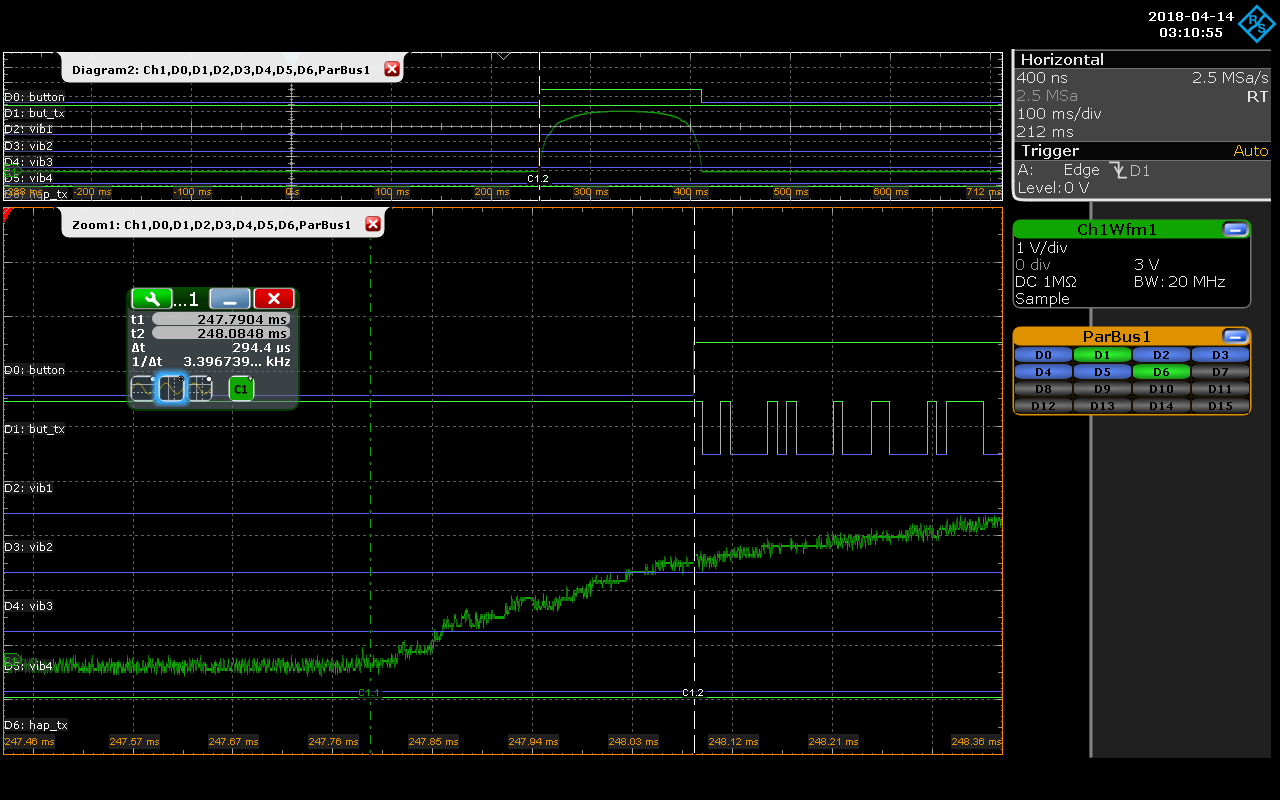
\includegraphics[width=\columnwidth]{buttonTX}
            \caption{FSR Button ramp up time before TX: 294.4 microseconds}
        \end{figure}
    \end{itemize}
    \item Haptic Device Latency
    \begin{itemize}
        \item In order to quantify latency within the haptic device tests were repeatedly run within a closed loop environment. This meant that the onset trigger I/O pin at the gate node of the Pro Trinket was connected to the A0 pin on the Arduino Uno, emulating the same effect as a tap of the FSR.
        \item The haptic test cases were run and the overall average asynchrony between true onset and tap onset across all test cases was found to be approximately -5 ms. The average on an individual test case basis would later be subtracted from the user test results to ensure fair results.
        \item A correction factor was necessary since the gate would open and trigger the tap before the onset at the end of motor 4. This time window changed based on the period and mode of operation.
        \begin{figure}[H]
            \centering
            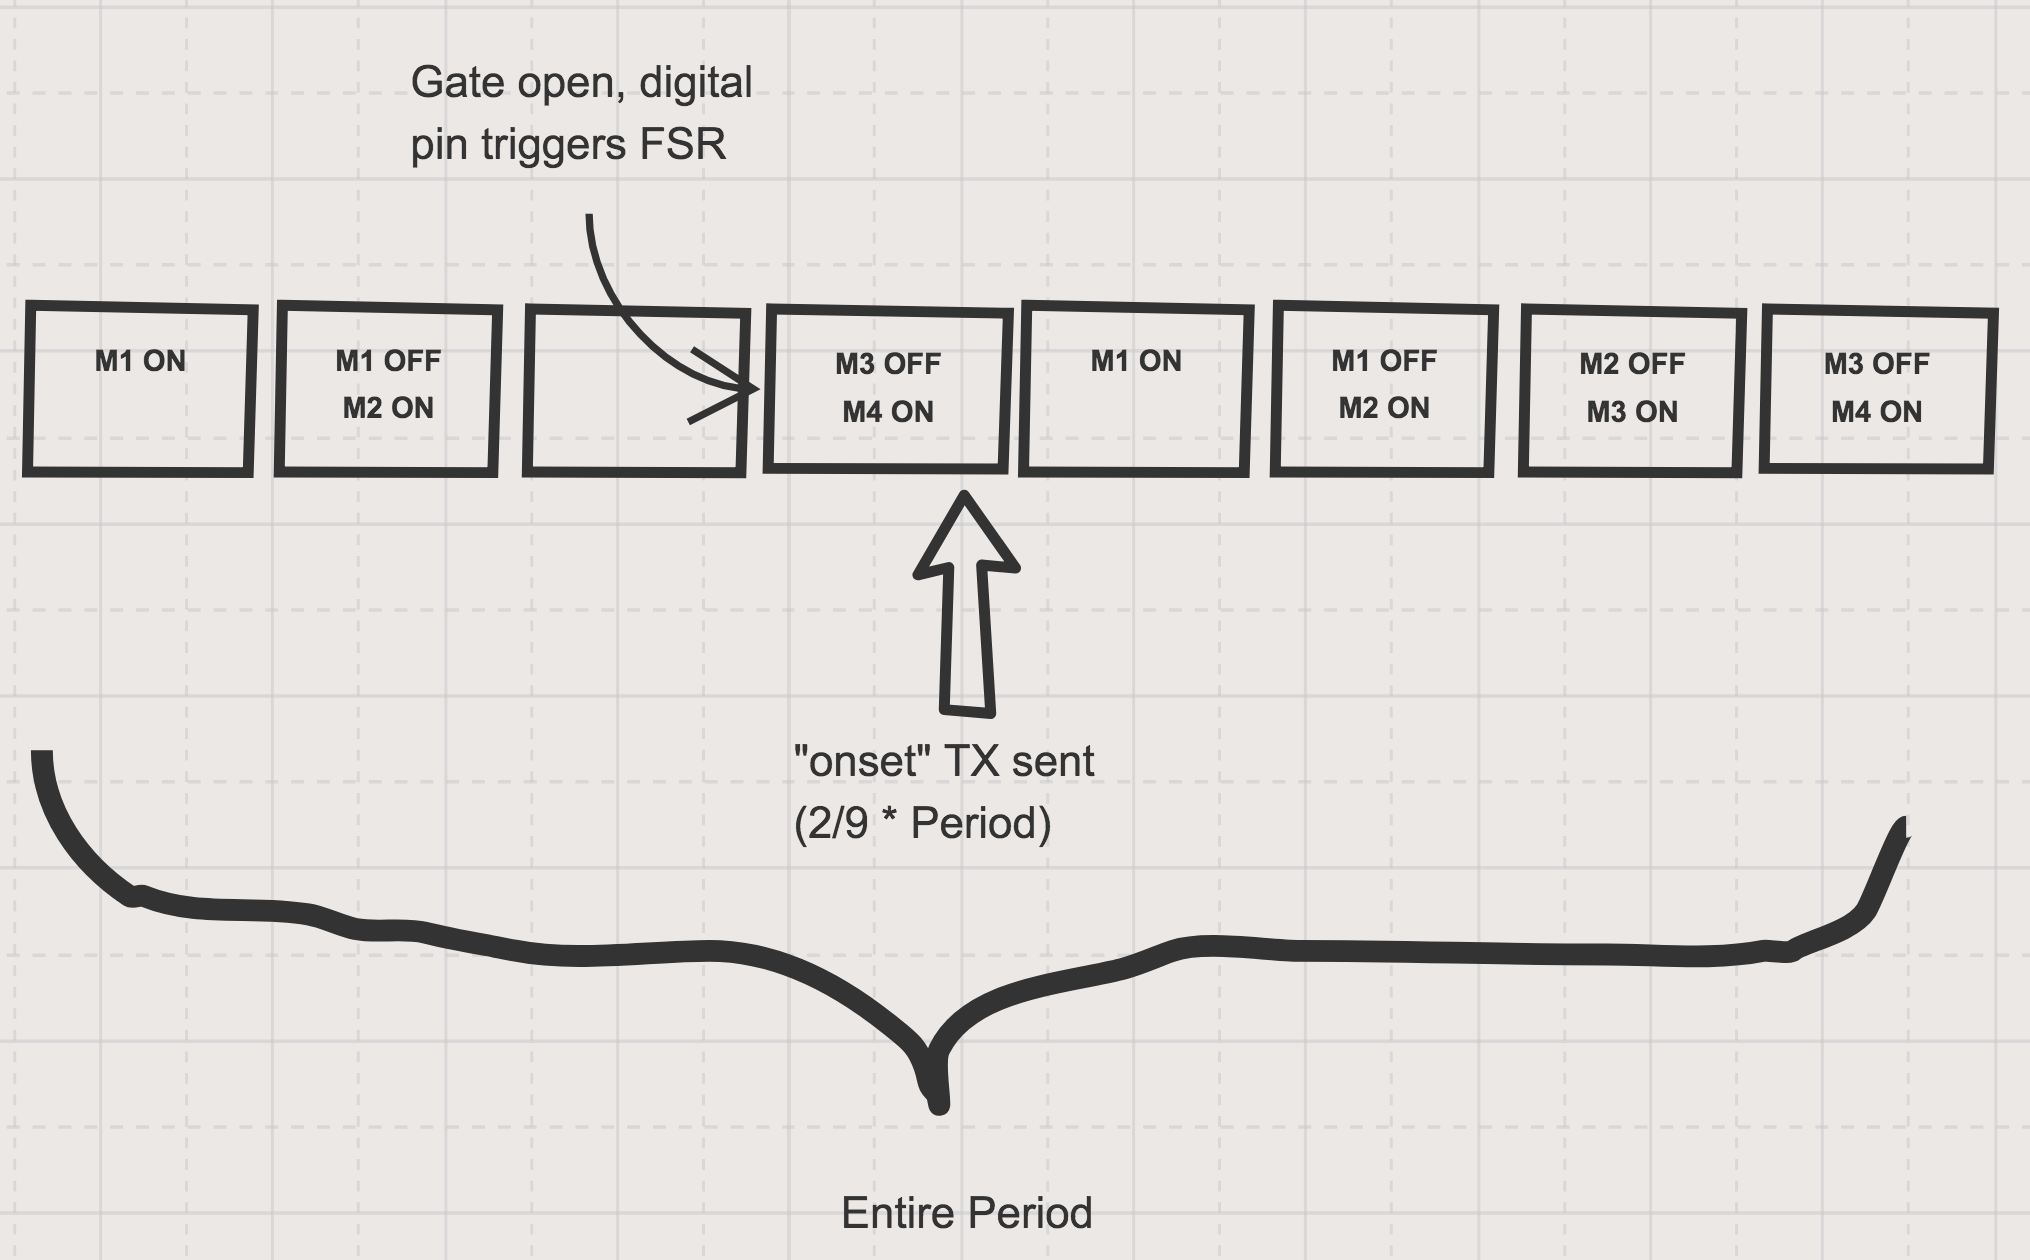
\includegraphics[width=\columnwidth]{diagramGateHaptic}
            \caption{Diagram of gate versus actual onset}
        \end{figure}
        \begin{itemize}
            \item Onset trigger in continuous mode 2/9ths (5/9-3/9) of the period. For a 1000 ms period the onset transmission does not occur until 2/9 * 1000 = 222.222 ms as confirmed in Figure \ref{hapticAdjustment}.
            \begin{figure}[H]\label{hapticAdjustment}
                \centering
                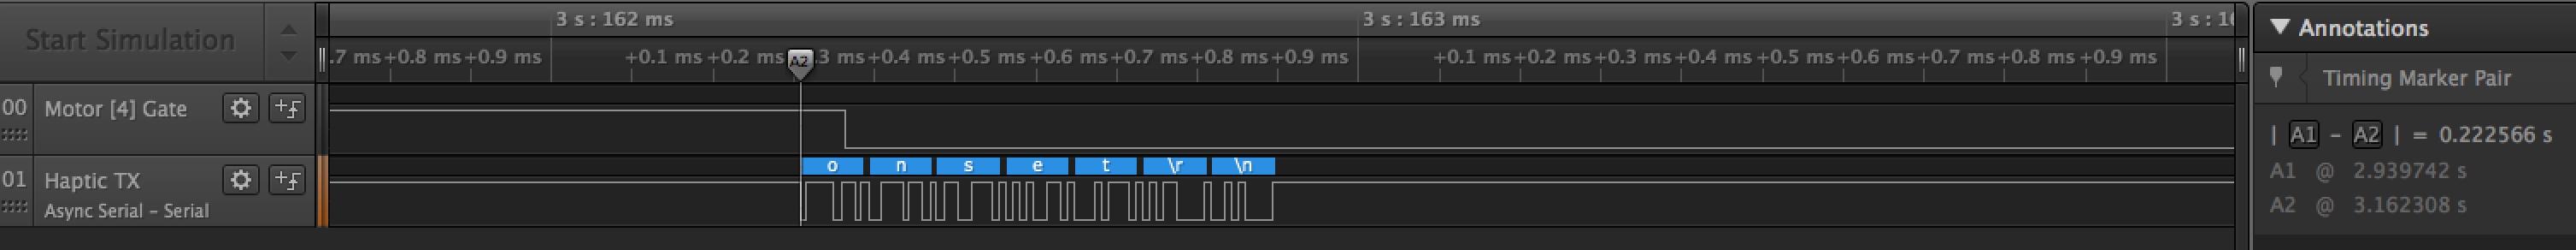
\includegraphics[width=\columnwidth]{hapticAdjustment}
                \caption{Haptic correction factor based on gate opening vs. actual onset message}
            \end{figure}
            \item The onset trigger in discrete mode starts $1/4$ of a period after.
        \end{itemize}
        % \item Additionally, research informs a 50 ms vibrotactile motor ramp up time to reach human perceptibility as confirmed in Appendix \ref{fig:MotorRampUp}.
    \end{itemize}
    \item Audio Latency
    \begin{itemize}
        \item Audio driver and sound card latency estimate of laptop\footnote{Mid 2012 Macbook Pro Retina 16GB RAM 2.6GHz i7}
        \begin{itemize}
            \item Tested via loopback method\footnote{\url{https://manual.audacityteam.org/man/latency_test.html}} with audio loopback dongle\footnote{\url{https://source.android.com/devices/audio/latency/loopback}} at 44.1 kHz 24 bit with an I/O buffer size of 64 samples. The resultant roundtrip latency was a negligible 3.4 ms.
        \end{itemize}
        \item Test system/Algorithmic latency (pyGame Audio library)
        \begin{itemize}
            \item A sound detector circuit was used which consisted of a electret microphone, preamp, envelope follower, and Schmitt trigger. The microphone sensitivity was calibrated to match the headphone input. The laptop output was shifted to a single channel such that it was only outputting from the left to avoid any time delay introduction from the right. 
            \begin{figure}[H]
                \centering
                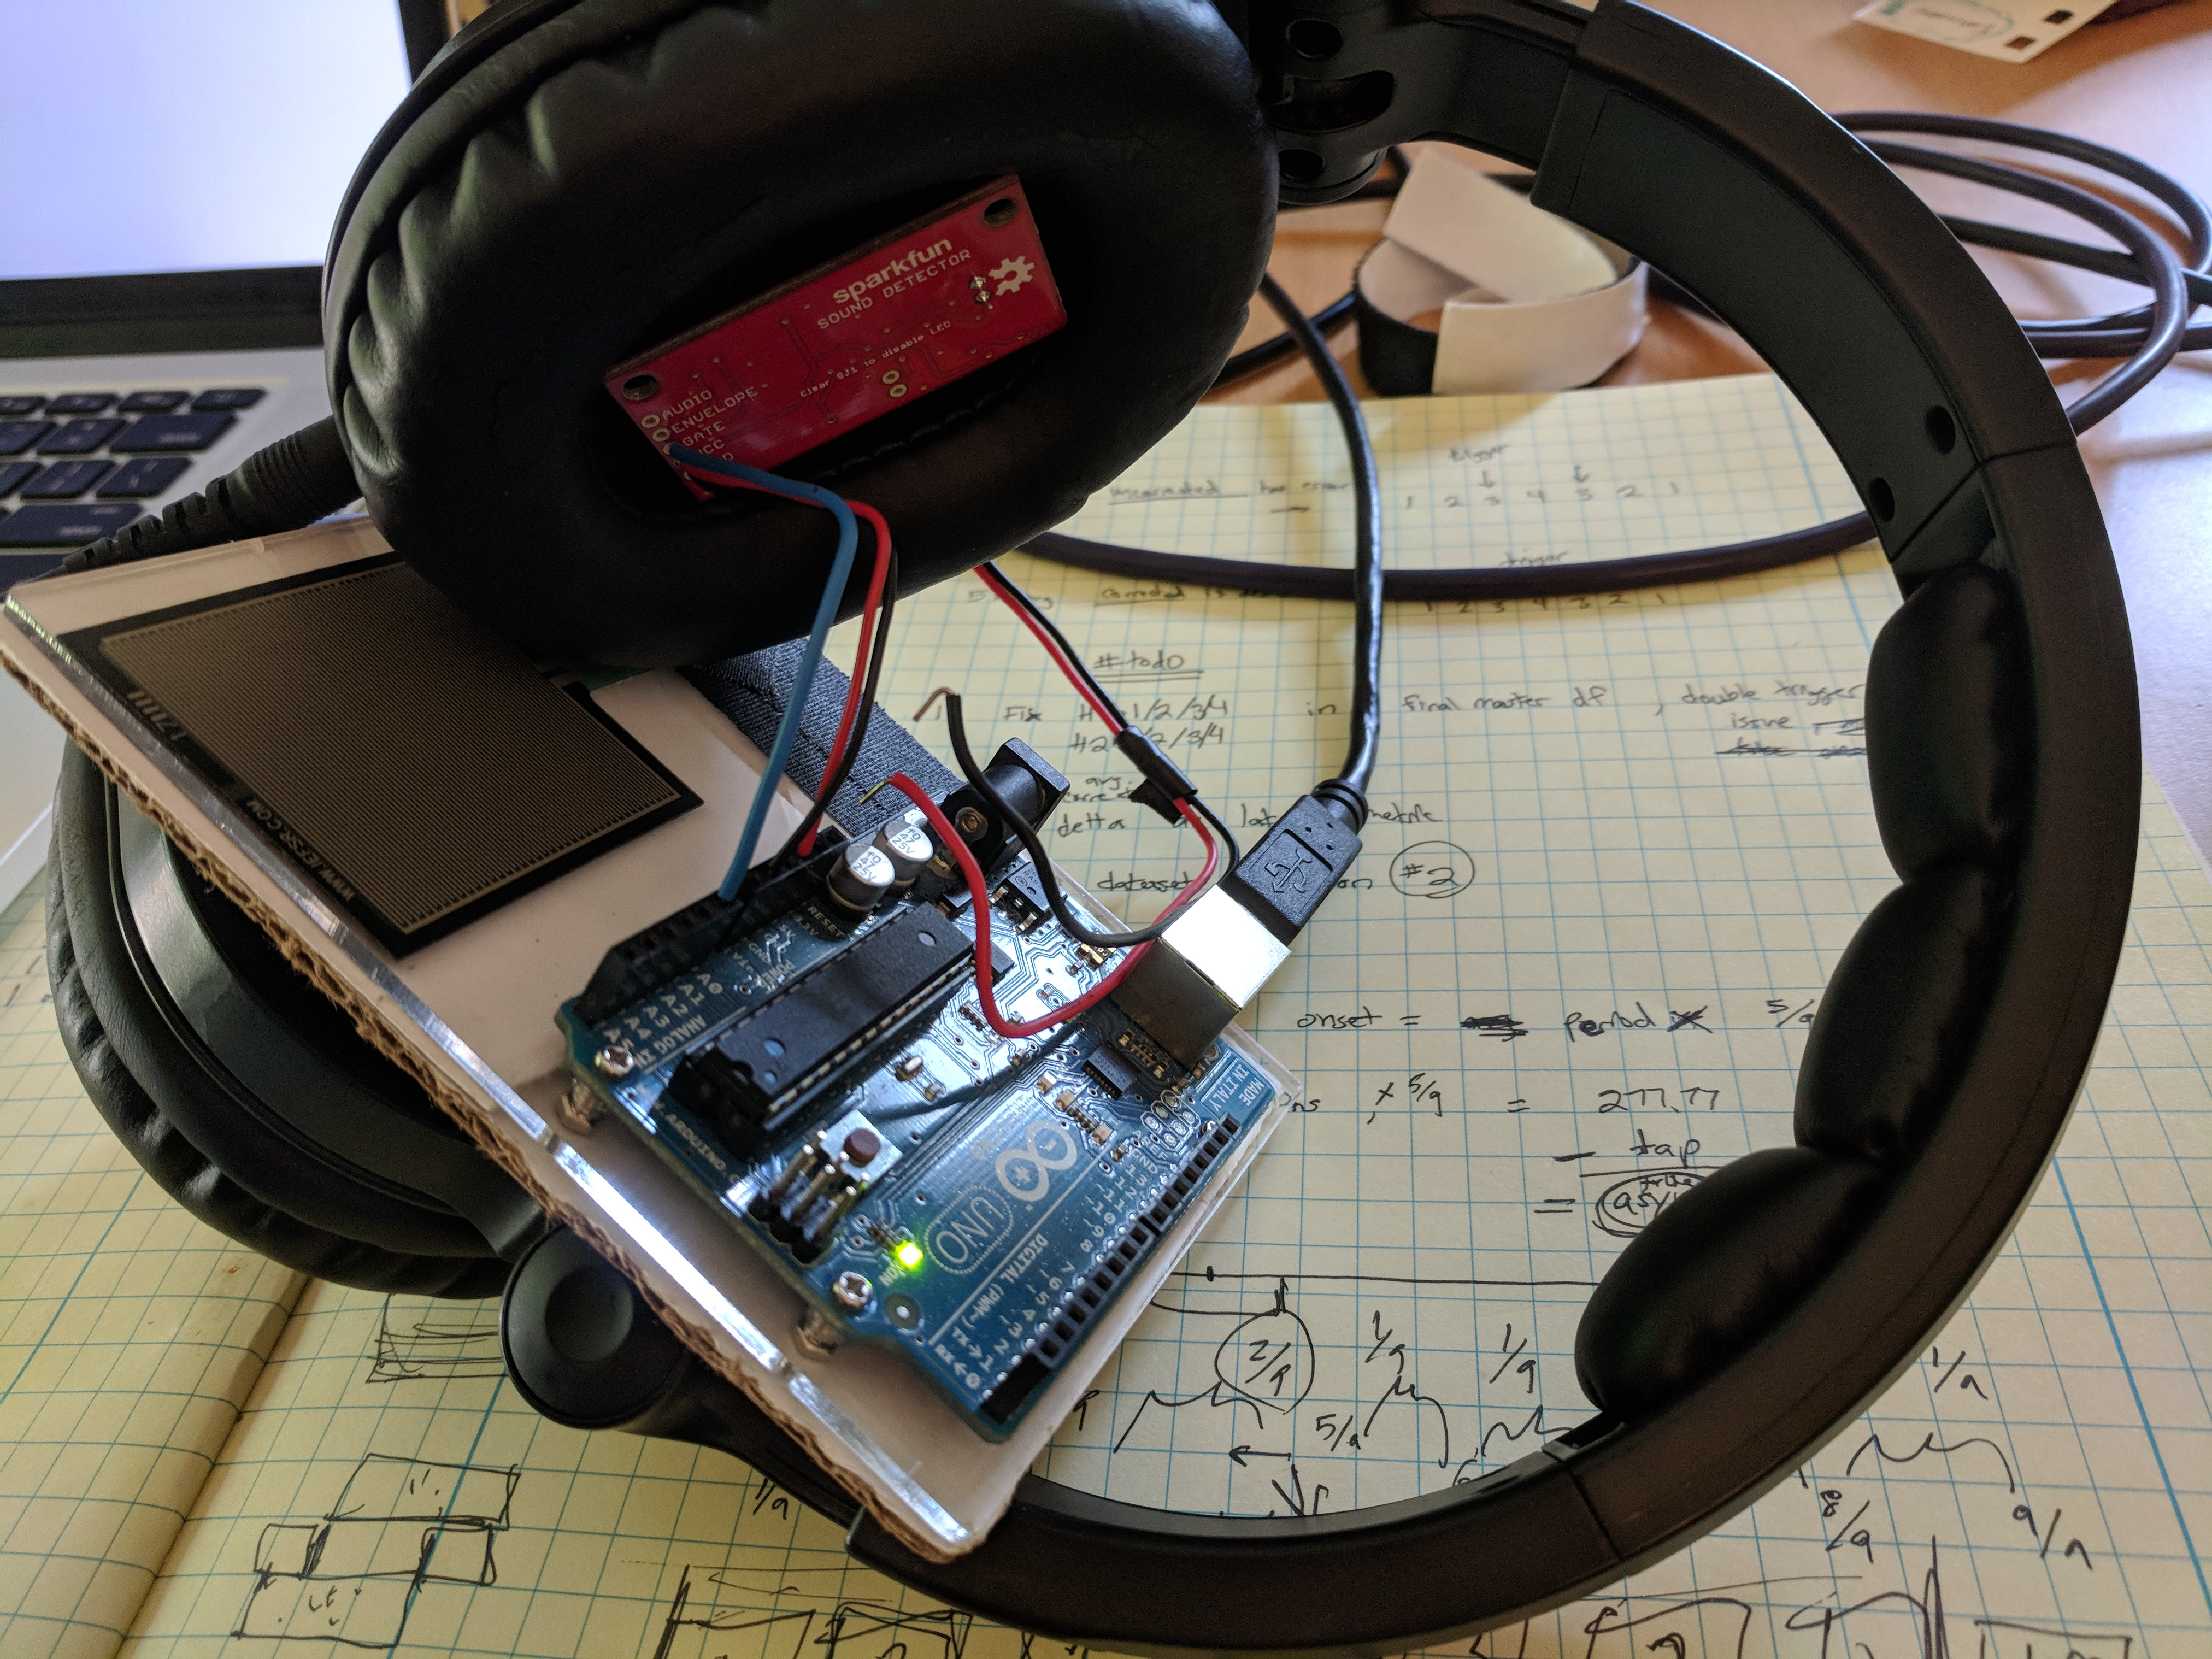
\includegraphics[width=\columnwidth]{AudioLatency}
                \caption{Audio Latency Setup}
            \end{figure}
            \item The gate pin of the sound detector was connected directly to the A0 input on the Arduino Uno. Any impulse exhibited by the headphones triggered the gate to output a digital signal. This triggered the Arduino identically to how the FSR registered a tap. 
            \item The audio test cases were run 5 times each. The discrepancy between true onset and tap onset represented the audible delay in the signal chain. This was averaged across all tests to equate to approximately 32.64 ms.
        \end{itemize}
    \end{itemize}
\end{itemize}
\subsubsection{Closed loop adjustments}
Although it was important to classify the magnitude of delay introduced by two simultaneous serial devices, the closed loop haptic and audible tests were the most crucial to compensate for which meant correction on an averaged per test case basis. Though this was applied to individual test cases, the overall for audible tests equated to an average reduction of 32.64 ms and for the haptic based tests an addition of 5 ms.